\documentclass[12pt,a4paper,leqno]{report}

\usepackage[ansinew]{inputenc}
\usepackage[T1]{fontenc}
\usepackage[english]{babel}
\usepackage{amsthm}
\usepackage{amsfonts}         
\usepackage{amsmath}
\usepackage{amssymb}
\usepackage{chemformula}
\usepackage{siunitx}
\usepackage{braket}
\usepackage{mathtools}
\usepackage{url}



\pagestyle{plain}
\setcounter{page}{1}
\addtolength{\hoffset}{-1.15cm}
\addtolength{\textwidth}{2.3cm}
\addtolength{\voffset}{0.45cm}
\addtolength{\textheight}{-0.9cm}

\title{The Chemical Path of Eroded Soil From Field to Bottom Sediment with Fe K-edge X-Ray Absorption Near Edge Spectroscopy.}
\author{Antti-Jussi Kallio}
\date{}

\begin{document}

\maketitle

\tableofcontents

\chapter{Introduction}\label{johd}
%
The state of Baltic sea has changed greatly during the past century. Baltic sea is connected to the Atlantic ocean via a rather small Danish straits. This means that the water body of the Baltic sea is nearly isolated and thus greatly affected by man made pollutions and nutrients. The eutrophication is one of the greatest challenges affecting the ecosystem and the population living around the Baltic sea. Poisonous blue green algae is a common sign of eutrophication, and large algae areas are common, as seen in figure. Large areas at the bottom of the Baltic sea are hypoxic, which along the nutrients accelerate eutrophication.

The main nutrients causing eutrophication are phosphorus and nitrogen. Fertilizers used in agriculture, waste waters and fallout from the atmosphere are the main sources of nutrients. The state of water systems around Baltic sea also affect the welfare of Baltic sea. Nutrients in lakes and rivers will ultimately emanate to the sea. Eutrophication causes increase in algae production, changes in the biocoenosis and in fish population, and also increase of hypoxic bottom waters. It is also tricky to control the eutrophication, since nutrients stored in bottom sediments can dissolve back to the water, even when if nutrient load is decreased.

\begin{figure}[h!]
   \label{fig:sinileva}
   \centering
      
\includegraphics[width=\textwidth]{../Kuvat/sinileva.png}
   \caption{Large blue green algae areas on the coast of Finland in July 2018 \cite{ymparisto}.}
\end{figure} 

The main source of nutrients is the agriculture. Two thirds of phosphorus release and over half of the nitrogen is coming from the agriculture \cite{helcom}. In our work we are focusing on phosphorus release from the bottom sediments. The phosphorus can be carried to the sea either by dissolving into the runoff waters, or by engaged in eroded soil, which is also carried by runoff waters. The eroded soil will at some point end at the bottom sediment of the sea, and face hypoxic conditions. Iron chemistry is closely related to phosphorus release in sediments. Iron oxides and \ch{SO4} are common electron acceptors in sediments, and the cycling of \ch{C}, \ch{Fe}, \ch{S} and \ch{P} is affecting the fate of \ch{P}. \ch{P} can be buried into the sediment, or released into the water in the cycling process. 

We will study the chemical evolution of \ch{Fe} from the field to the water, and ultimately to bottom sediment and hypoxic environment. In order to study the chemistry, we are using X-ray absorption spectroscopy, particularly the X-ray absorption near edge spectroscopy, XANES. This element specific technique is sensitive to the chemical state of the element of interest. We will also develop a measurement method to study the mix of sediment and sea water, which is also possible to be used in anaerobic sample preparation. We'll also compare are measurements known reference samples, and with the knowledge of sediment chemistry we can try to estimate the phosphorus release.

If our measurement technique turns out to be usable, and we are also able to obtain meaningful results, our technique can be used to study larger set of samples and also chemistry of other elements in the soils. With further studies one can form a better picture of the sediment processes, and their effect on eutrophication. This knowledge can be used to form new guidelines for farmers on erosion control measures and phosphorus control measures. Our results can also be applied to other water bodies, affected by eutrophication, not just the Baltic sea.

This work is done with co-operation of Finnish Environment Institute and Physics Department of University of Helsinki, and is part of a large Samassa Vedess� study \cite{samassa}.       

\chapter{Phosphorus and Iron Cycling in the Aquatic System }\label{phosphorus}


\section{Soil as a Carrier of \ch{Fe} and \ch{P}}\label{Soil}
The release of soil, \ch{Fe} and \ch{P} from the fields or from other terrestrial sites and their transport to the aquatic system is well known and defined process. Iron contributes 5.1 mass percent of the earth's crust \cite{?} and is a major component of many soil-forming parent materials. The concentration of \ch{Fe} in surface soil is on average $3.5\%$ \cite{Fe concentration}, and the concentration is a function of soil characteristics. In Finland the concentration varies between $1.6-7.1\%$ in post-glacier soils \cite{Fe concentration}. On the other hand the more weathered soils for example in Guadalquivir Valley in Spain the \ch{Fe} concentration is measured as low as $0.9\%$ \cite{Soil erosion}. The concentration of \ch{Fe} in eroded soil thus reflects the concentration of the parent soil, thought the concentration might be modified by selective erosion, for instance, fine particles. Half of the \ch{Fe} in riverine particles consists of largely inert \ch{Fe} silicates, and the other half is possibly reducible forms like oxides \cite{Soil erosion}.

For the sake of simplicity we will call the oxides, hydroxides and oxide-hydroxides of \ch{Fe}(III) as \ch{Fe} oxides. These oxides are common all around the environment, with varying concentrations between one to several hundred $\si{\gram\per\kilo\gram}$ in aerobic soils. They also exist in variable forms, with different mineralogy, crystallinity, grain size, etc, which affects the the availability and chemical reactivity of the \ch{Fe} oxides. The age of the soil also affects the available \ch{Fe} oxides. For example in warmer and dryer climates with older soils, the \ch{Fe} oxides are often present in crystalline form. On the other hand on boreal conditions the \ch{Fe} oxides are often in poorly crystalline form. The poorly crystalline forms have high capacity to absorb \ch{P} in neutral pH. \ch{Fe} oxides can also be bound by organic \ch{C}, which can carry the \ch{Fe} to aquatic system \cite{Soil erosion}. 

Both \ch{Fe} and \ch{P} are naturally present in soils, but the use of chemical fertilizers have increased the reserves of \ch{P}. The increase of \ch{P} reserves has been made possible by the high ability of \ch{Fe} and \ch{Al} to capture \ch{P} by ligand exchange reactions. The \ch{P} rich surface soil is extracted in erosion processes and transported to water bodies. \ch{P} is released in the aquatic system due to changes in ionic composition. 

Rivers transport $13-19 \si{\peta\gram}$ of suspended solids to the oceans per year. Most of the solids settle out to become sediments in estuary and coastal regions. Total yearly flux of \ch{Fe} is $960 \si{\tera\gram}$  and \ch{Fe} oxides is $270-430 \si{\tera\gram}$, mainly as small particles which also settle to be estuary. \ch{P} flux is estimated to be $18-30 \si{\tera\gram}$ yearly, of which 25-45\% is expected to be reactive \cite{}.  

Particulate \ch{P} erosion is affected by tillage depth, intensity of tillage, plant coverage, soil texture, soil quality, slope and hydrology. The amount of \ch{P} losses are thus highly variable and the type of arable land is the main variable. Particulate \ch{P} is often dominant in runoff from fine-textured soils without permanent plant cover. In Scandinavia up to 93\% of total \ch{P} is in particulate form in agricultural runoff. The algea needs \ch{P} in dissolved orthophosphate form, so \ch{p} needs to be released from particles. Algae studies have shown that in eroding river banks only less than $1-13\%$ of \ch{P} and in lake banks no \ch{P} was available. On the other hand in agricultural rivers the availability of particulate \ch{p} ranges from 5 to 41\% with norm somewhere between $20-30\%$.

If we assume $20-30\%$ of the particulate \ch{P} to become available in receiving waters, we may assume the losses of bioavailable particulate \ch{P} to be at similar level. 

With the previous calculations the current erosion control measures seem appropriate. However they do not take into account any sediment processes, which are the main focus in our research.                        
% Lannoittamisesta

% Jokien kuljetuksesta

% fosfori h�vi�t pelloilta

% 

\section{The Role of Sediment}\label{Sediment}
The existing literature on phosphorus cycling focuses on the link between soil erosion and \ch{P} transport, or \ch{P} bioavailability. However at some point the particles have become part of the sediment and eventually they will face anoxic environment, which has an impact on \ch{Fe} cycling, and thus also affect the fate of \ch{P}.

The sediments reduce \ch{Fe} oxides via two distinct processes. The first one is called microbial dissimilatory \ch{Fe} reduction, where the microbes use the oxides as terminal electron acceptors in respiration. In the other process the oxides are reduced chemically by oxides formed in microbial \ch{SO4} reduction. For both of these methods the primary energy source for reduction is organic \ch{C}. The flux of organic \ch{C} to the bottom surface decides the dominant mode of reduction. In case of low \ch{C} flux the sediment has plenty of \ch{Fe} oxides, and the \ch{Fe} reduction is often the dominant process. When the eutrophication increases also the settling flux of organic \ch{C} increases. This causes the \ch{Fe} reduction to give way for \ch{SO4} reduction. Due to this change in sediment microbiological processes, the state of the entire ecosystem may be altered. Sediment may no longer be able to retain \ch{P} due to \ch{SO4} reduction taking place. The available \ch{Fe} oxides are able to constrain \ch{SO4} reduction. As previously deicussed, the \ch{Fe} oxides in marine waters are mainly carried from terrestial lands. However the role of soil erosion in transport of \ch{Fe} oxides for benthic mineralization, and possibly lowering of benthic \ch{P} fluxes, has been poorly studied. 

For decades we have known the relation between greater primary production and high concentrations of \ch{SO4} and the increase in \ch{P} production. \cite{?}. The underlying mechanisms however have only recently been cracked. \ch{Fe} cycling has rather different consequences depending on type of \ch{Fe} reduction. If the \ch{Fe} oxides are reduced by microbial dissimilatory reactions and produce highly soluble \ch{Fe}(II),which is able to diffuse upward in the pore water. Ultimately the \ch{Fe}(II) will be oxidized by e.q. \ch{O2} or \ch{NO3}. These newly formed \ch{Fe} oxides will form a layer, which is able to capture \ch{P}, and also diffuse upward in the sediment. If the bottom fauna mixes the surface of the sediment, an individual \ch{Fe} atom can can be re-used hundreds of times in microbial mineralization reactions, which is also known as "a ferrous wheel". The "ferrous wheel" is able to take large part of anaerobic respiration and also lower the pool of labile \ch{C} for \ch{SO4} reduction and \ch{CH4} formation.

Microbial reduction can only partly reduce the crystalline \ch{Fe} oxides, but that's not the case for sulfides. The sulfides are able to fully reduce the crystalline \ch{Fe} oxides, and furthermore produce insoluble \ch{Fe} sulfides. This will result in \ch{Fe} to be in solid form and buried in sediment.  No \ch{Fe} will be able to diffuse upward to form oxide layer on the sediment surface, and \ch{P} is no longer bound with \ch{Fe}. 

\section{The Effects of \ch{C}/\ch{Fe} Ratio}\label{c/fe}
The effects of \ch{C}/\ch{Fe} ratio has been studied by performing long-term incubations on field soil to simulate the conditions that eroded soil encounters in an estuary and in brackish sediment by Lehtoranta et al. \cite{}. It was noted that the release of \ch{P} was coupled with the release of \ch{Fe}. When organic \ch{C} was not present. This indicates that microbial \ch{Fe} reduction is causing both \ch{Fe} and \ch{P} to accumulate into \ch{Fe} minerals. This means that \ch{Fe} is able to bind \ch{P}, when in an oxic environment. When the amount of organic \ch{C} was increased, it decoupled the cycles of \ch{Fe} and \ch{P}, since the \ch{SO4} reduction started to take place. This resulted in the release of \ch{P} into the water. It was also noted that the color of the sediment turned black, indicating that \ch{Fe} sulphides were formed in the process.

In our study we are performing similar incubations and trying to gain deeper knowledge of the chemical changes in these systems. For example the color change can be a result of a rather small increase of \ch{Fe} sulphides in the system, and we try to verify large the increase actually is. 

\section{The Effects of Eroded Soil on Eutrophication}\label{Outline}
The effects of eroded soil on eutrophication in \ch{SO4} rich water body is the main interest of our research. The sediment processes are not well known, but Ekholm et all have proposed an outline \cite{Soil erosion}, which will be discussed in this section.

If the estuary is under heavy riverine input of \ch{Fe} oxides and modest input of dissolved \ch{P}, it is expected to show only moderate level of eutrophication, as shown in figure \ref{fig:eutroA}. Due to low level of dissolved \ch{P} the planctonic algae etc. are not able to produce high amounts of \ch{C} and due to the high input of \ch{Fe} oxides, the settling flux has high \ch{C}/\ch{Fe} ratio. In this case the if the dissolved \ch{P} is reduced by load control measures the estuary may respond positively due to the coupled cycling of \ch{P} and \ch{Fe}. In an environment like this the benthic fauna is prosperous and the "ferrous wheel" is in action.  
\begin{figure}[h!]
  \label{fig:eutroA}
  \centering
  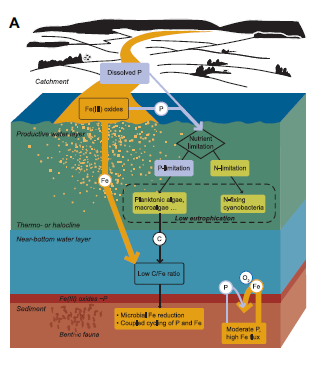
\includegraphics[width=0.8\textwidth]{../Kuvat/eutrophication_A.png}
  \caption{Expected effects of eroded soil on eutrophication on estuary in case of high amount of \ch{Fe} oxide flux \cite{Soil erosion}.}
\end{figure}

If erosion control measures takes place in the catchment of an estuary, we might see a decrease of \ch{Fe} oxides due to lowered flow of soil, but an increase in dissolved \ch{P}. The increase of \ch{P} is common outcome of reduced tilling. The increased amounts \ch{P} triggers algal production, which increases the flux of organic \ch{C} to the sediment surface. As the amount of \ch{C} increases the \ch{SO4} reduction becomes more important. The reduction in the \ch{Fe} oxide flux further promotes the importance of \ch{SO4} reduction as the \ch{C}/\ch{Fe} ratio is increased. As \ch{SO4} reduction rate increases, more of the sediment \ch{Fe} is transformed into non-sorptive \ch{Fe} sulfides. Now the "ferrous wheel" is broken and \ch{Fe} bound \ch{P} stored in sediments is released causing the estuary to be highly eutrophic. The benthic fauna of the sediment is largely gone and we might observe large cyonobacterial blooms. This state is difficult to reverse, due to the requirement of a shift in sediment microbial processes and a successful load reduction. This outline is visualized in figure \ref{fig:eutroB}.
\begin{figure}[h!]
   \label{fig:eutroB}
   \centering
   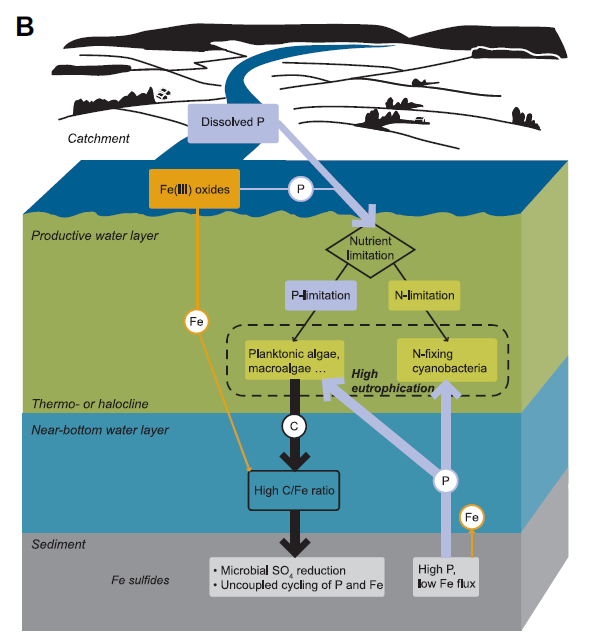
\includegraphics[width=0.8\textwidth]{../Kuvat/eutrophication_B.png}
   \caption{Expected effects of eroded soil on eutrophication on estuary in case of low \ch{Fe} oxide flux \cite{Soil erosion}}
\end{figure}

The effect of increase in \ch{C} production, caused by \ch{P}, are not straight forward. The settling flux is affected by the hydromorphology and chemistry of the receiving water body. For example in deep systems the \ch{C} is largely mineralized in water phase, and benthic processes are almost non-existent. The depth profile also affects sediment accumulation. Lastly any barriers in \ch{O2} transport to near bottom waters, such as thermocline and halocline, affect the sediment state. 

The availability of \ch{SO4} is obviously crucial for sediment processes. With low \ch{SO4} levels, the \ch{SO4} reduction plays only minor role. The \ch{P} can be expected to be desorbed in soil particles, in addition to \ch{P} in dissolved form.

If eroded soil improves the ability of the soil to preserve the \ch{P} by promoting \ch{Fe} reduction and later by coupled \ch{Fe} and \ch{P} cycling, the net effect on eutrophication depends on the balance of following factors:
\begin{enumerate}
\item Labile soil \ch{P} that can support algal primary production.
\item The lowering of benthic \ch{P} release caused by \ch{Fe} oxides.
\end{enumerate}
The balance is evidentially site-spesific, but it is possible to estimate it by determining the rate of \ch{Fe} that is available for \ch{Fe} reducing microbes and also by determining rate of dissolved \ch{P}.

\section{Vivianite}
Another major component affecting the fate of \ch{P} is hydrated iron phosphate called vivianite ($\ch{Fe3(PO4)2*}8\ch{H2O}$). The long-term storage of phosphorus in marine systems is in sediments. Phosphorus retention in sediment is however limited by the redox dependency. Organic phosphorus under anoxic conditions is remineralised faster relative to organic carbon and iron-oxyhydroxides, bearing phosphorus, undergo dissolution \cite{}. The efflux of phoshorus from the seafloor can have negative impact on eutrophication.     

In Baltic sea the removal of phosphorus mostly caused by burial of organic matter. However recent observations have shown that vivianite may act as major sink for phosphorus, as it is buried into the sea bottom \cite{}. Most commonly the precipitation of vivianite observed with high concentrations of pore water iron in the absence of hydrogen sulphite, such as below the sulphate-methane transition zone \cite{?}. Nonetheless recently vivianite has also been observed within the sulphate-methane transition zone in Baltic sea sediments \cite{}. The possible cause of the observation was presented by Reed et al in their simulation study \cite{?}, and their scenario is summarised in figure \ref{fig:vivianiitti}.

\begin{figure}[h!]
  \label{fig:vivianiitti}
  \centering
  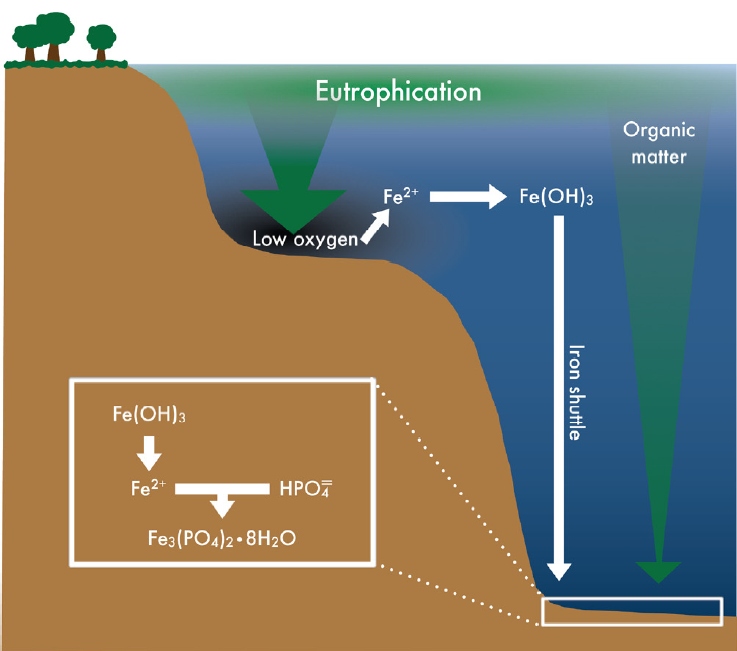
\includegraphics[width=0.8\textwidth]{../Kuvat/vivianiitti.png}
  \caption{The outline of vivianite production in sediments \cite{?}.}
\end{figure}

Their simulation was based on sediment samples taken from one of the deep sea basins of Baltic sea, where oxic and anoxic conditions alter based on major inflow events of dence oxic water from the North Sea. 

As a result they noticed that the amount of vivianite found in the sediment was a function of the iron flux settling to the bottom. However the \ch{P} can also be bound in other iron oxyhydroxides, but the vivianite might be one component to look for, when performing the analysis of our samples.    
    

\section{The Sediment as a Research Interest}
In this research we are using x-ray absorption spectroscopy to study the sediments in different environments and try to verify if we are able to see any shifts in chemical environment. We try to simulate the path of the soil by first measuring the spectra of different soil types, which have been dried and filtered. Then we are going to mix the soils with estuary waters and vary the level of labile organic \ch{C} and \ch{S}. Lastly we introduce an anaerobic environment. The absorption spectra will be measured in each case and we try to trace whether there is a shift in the chemical state or not. We are expecting the chemical state to remain similar during the two first experiments and in the third one according the outline described in section \ref{Outline}, we are expecting to see an increase of \ch{Fe} sulfides in our samples.

If our method of sediment research works, it can be applied to measure large set of different water and soil types to further study the effects of soil erosion and agriculture in different water types.

\chapter{X-ray Absorption Spectroscopy}\label{XAS}
X-ray absorption spectroscopy (XAS) focuses on studying how x-rays are absorbed above and below the element specific jumps in the absorption cross-section called absorption edges. XAS allows studying of the local structure around selected element in the sample. XAS does not require long range order, and it can be applied not only to crystals, but to amorphous systems, glasses, quasicrystals, disordered films, membranes, solutions, liquids, metalloproteins, molecular gases etc. These multiple measurement systems make XAS versatile tool in various different fields, such as physics, chemistry, biology, medicine, engineering, environmental science and geology.

X-ray absorption measurements are relatively straightforward. The main difficulty is obtaining a energy-tunable x-ray source. Traditionally this has meant synchrotron radiation sources, but lately laboratory systems based on analyzer crystals have gained some ground due to limited synchrotron beam time and due to price drop of the crystals. Many experimental techniques and sample conditions can be applied in XAS measurement, where the most limiting factors are often the energy range, beam size and intensities available from the x-ray source.  

The term "XAS", also known as "XAFS" (X-ray Absorption Fine Structure), is an upper level term for various techniques. XAS is typically divided into the XANES (X-ray Absorption Near Edge Spectroscopy) region, which focuses on the energies at vicinity of the absorption edge, and the EXAFS (Extended X-ray Absorption Fine-structure Spectroscopy), which focuses on the energies well above the absorption edge.

\section{X-ray Absorption and Fluorescence} 
X-rays are a form of electromagnetic radiation. Typical X-ray energies range from $\sim 500 \si{\electronvolt}$ to $500 \si{\kilo\electronvolt}$, and wavelengths from $\sim 25 \si{\angstrom}$ to $0.25 \si{\angstrom}$. In typical X-ray energy range, the photons are absorbed by matter through photo-electric effect. Electrons are bound in atoms with discrete energies. When an incoming X-ray photon hits an atom, the photon can either excite or remove an electron. In order for an electronic core-level to participate in absorption, the x-ray photon has to have energy equal or greater than the binding energy of core level electron.  Released electron is called photo-electron. Right at   In photo-electric effect an X-ray photon is absorbed by an electron in a tightly bound quantum core level of an atom.

 
  %absorptiokerroin
In XAS measurement the basic physical quantity to measure is the x-ray absorption coefficient $\mu(E)$, which describes the probability that x-rays will be absorbed as a function of energy. Typically the $\mu(E)$ decreases smoothly as energy is increased, approximately as $1/E^3$ \cite{?}. However there are sudden jumps in the absorption cross-section at certain energies. These jumps are characteristic of the atoms in the materials and they occur when the x-ray photon has equal energy to that of the binding energy of a core-level electron, and they are called absorption edges. 

The absorption coefficient can be obtained from Beer's law:
\begin{equation}\label{eq:beer}
I=I_0e^{-\mu x} \Rightarrow \mu(E)= ln{\frac{I_0}{I_x}}, 
\end{equation}
where $I_0$ is the intensity of x-rays incident on a sample, $x$ is the sample thickness and $I$ is the intensity transmitted through the sample.   
For most x-ray energies the absorption coefficient is a smooth function of energy
\begin{equation}
\mu\approx\frac{\rho Z^4}{AE^3},
\end{equation}
where $E$ is the x-ray energy, $\rho$ the sample density, $\Z$ the atomic number and $A$ the atomic mass.

%mu ja Z riippuvuus
Absorption coefficient is strongly dependent on both $Z$ and $E$. $Z$ dependence allows the contrast between materials with different densities in typical X-ray image. The $E$ dependence on the other hand allows to obtain a suitable penetration depth into the material, by adjusting the beam energy. These features are useful in medical and other imaging techniques.
%absorptioreuna

As previously stated, there is a sharp rise in absorption when the incident X-ray energy is equal to the binding energy of a core-level electron, which is called the absorption edge. When performing a XAS measurement we are interested in the intensity of $\mu$ as a function of energy at the vicinity of the absorption edge. Every atom has well-defined core-level electron binding energies, so in XAS one can select the element of interest by altering the x-ray energy to an appropriate absorption edge. Typically $K-$ or $L-$edges can be measured at soft-X-ray beamline and both $K-$ and $L-$ edges at hard-X-ray beamline ($M-$edges for heavy elements can be measured at soft-X-ray beamlines). The edge energies vary with atomic number approximately as $Z^2$, allowing most elements to be measured with x-ray energies between $5-35\si{\electronvolt}$. 
%viritetty tila
After the atom has absorbed the X-ray photon, the atom is in excited state. In the excited state atom has one of its core electron levels empty, and a photo-electron. After the absorption event the excited state will typically decay within a few femtoseconds. The core hole can decay by two different absorption processes. The first one is X-ray fluorescence, where higher energy electron fills the core hole, and characteristic X-ray is emitted. These well-defined X-rays are characteristic to the atom and are tabulated. X-ray fluorescence can be used to identify atoms and quantify their concentrations. The second process for the decay is the Auger effect. In the Auger effect an electron falls into the vacancy and the energy is transferred to another electron, which is ejected from the atom into the continuum. X-ray fluorescence is occurring more often in the hard X-ray measurement than the Auger effect, and in case of soft X-rays Auger effect is more probable. Absorption coefficient $\mu$ can be measured using either these processes.        

%transmissio ja fluoresenssi
XAS measurement can be done by using transmission or fluorescence geometries. Transmission, which we are using in our measurements is further discussed in section \ref{transmission}. In transmission geometry we can measure energy dependence of absorption coefficient $\mu(E)$ as 
\begin{equation}\label{eq:transmissio}
\mu(E)=\log(I_0/I) 
\end{equation}
or in fluorescence geometry as 
\begin{equation}\label{eq:fluorescense}
\mu(E)\propto I_f/I_0
\end{equation}
where $I_f$ is intensity of a fluorescence line.


XAS spectra can be divided in two distinct portions as seen in figure \ref{fig:xassections}. The spectra shows a sharp rise of $\mu(E)$, which is due to $1s$ to $(n+1)p$ transition, and the oscillations of $\mu(E)$, which are the fine-structure. The XANES portion of the spectra is typically within $30\si{\electronvolt}$ of the main absorption edge and the EXAFS portion. EXAFS region extends typically $500-1000\si{\electronvolt}$ from the XANES portion. EXAFS portion can be interpreted more quantitatively due to some important approximations and limits.  
\begin{figure}[h!]
   \label{fig:xassections}
   \centering
   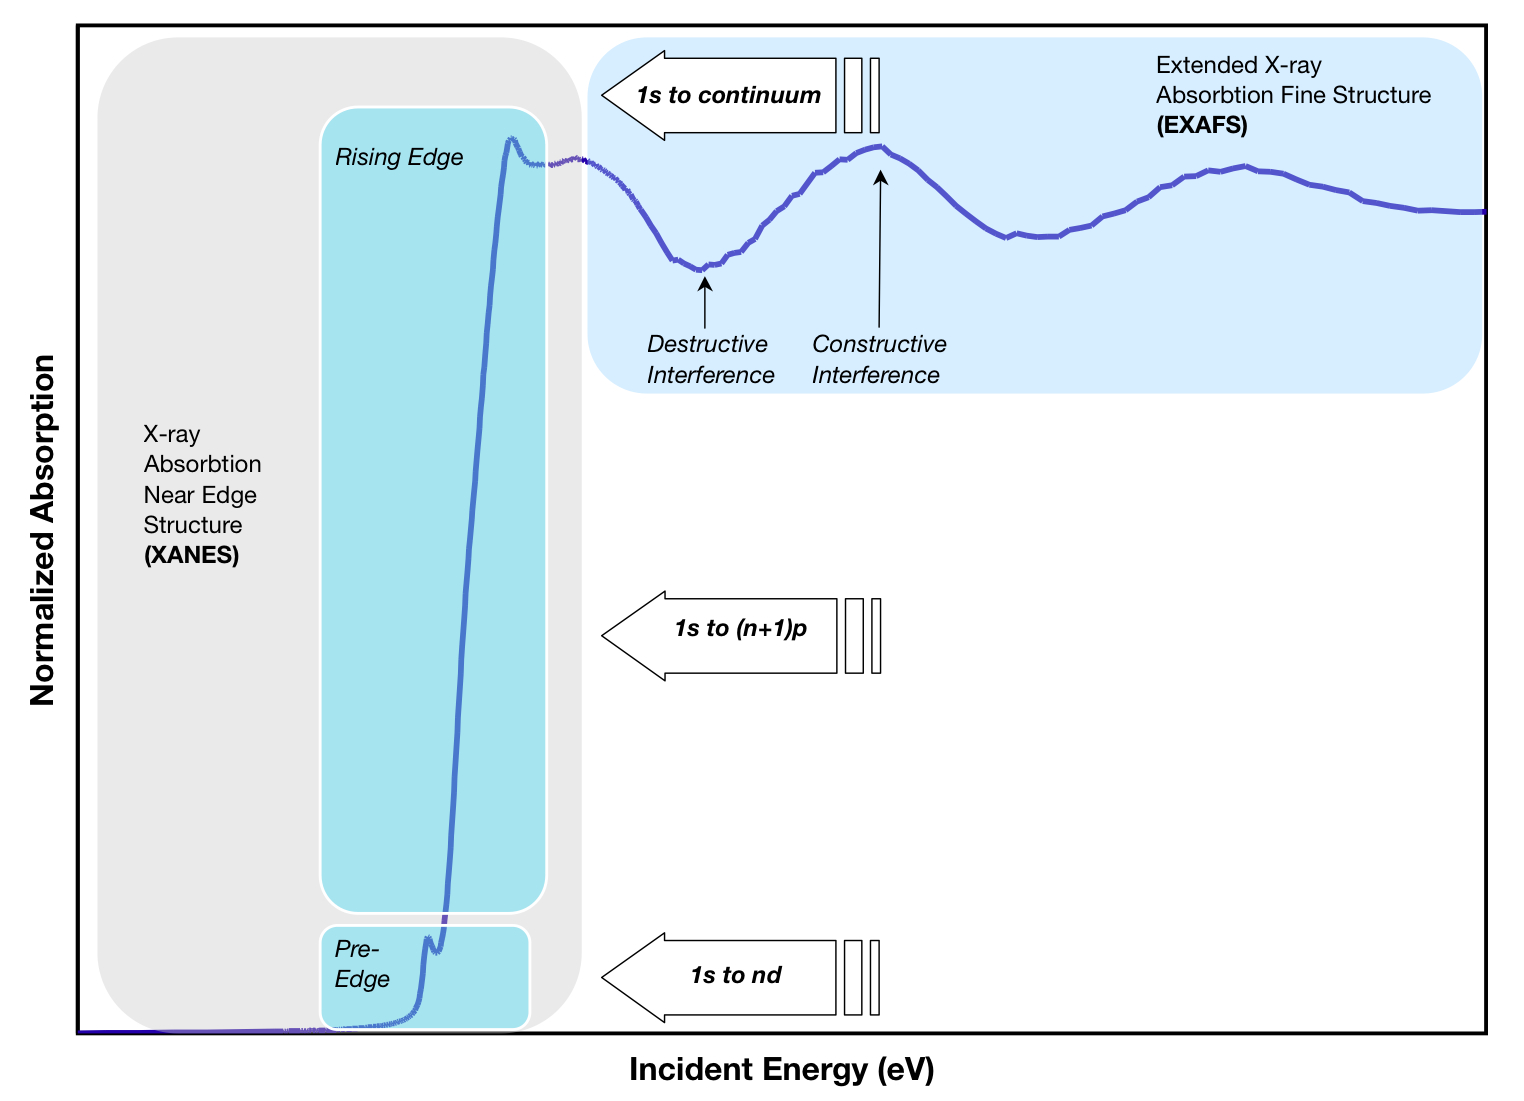
\includegraphics[width=\textwidth]{../Kuvat/XASFig.png}
   \caption{Sections of a typical XAS spectra \cite{?}}
\end{figure}

%In EXAFS the main interest are the oscillations well above the absorption edge. The EXAFS fine-structure $\chi(E)$ is defined as 
%\begin{equation}\label{eq:fine-structure}
%\chi(E)=\frac{\mu(E)-\mu_0(E)}{\Delta\mu_0(E_0)}
%\end{equation}
%where $\mu(E)$ is the measured absorption coefficient, $\mu_0(E)$ is a smooth background function describing the bare atom absorption and $\Delta\mu_0$ is the measured jump in the absorption $\mu(E)$ at the threshold energy $E_0$ as seen in figure \ref{fig:typicalxas}.

%\begin{figure}[h!]
%   \label{fig:typicalxas}
%   \centering
%   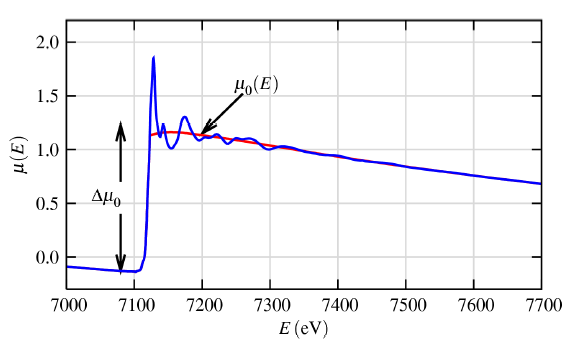
\includegraphics[width=0.7\textwidth]{../Kuvat/xastypical.png}
%   \caption{Smooth background function $\mu_0(E)$ and height of the edge step $\Delta\mu_0(E_0)$}
%\end{figure}

%Instead of photon energy $E$, it is common to use the wave number $k$ of the photo-electron 
%\begin{equation}\label{eq:k}
%k=\sqrt{\frac{2m(E-E_0)}{\hbar^2}}
%\end{equation}
%where $E_0$ is the absorption edge energy and $m$ is the electron mass. The main interest in EXAFS is thus the oscillations as a function of wave-number: $\chi(k)$. $\chi(k)$, often called as "the EXAFS", decays quickly with $k$. The oscillations can be emphasized by multiplying by a power of $k$.

%Different near-neighbour coordination shells correspond to different frequencies observable in the oscillations of $\chi(k)$. This can be modelled by the EXAFS equation: 
%\begin{equation}\label{eq:EXAFS}
%\chi(k)=\sum_j\frac{N_jf_j(k)e^{-2k^2\sigma_j^2}}{kR_j^2}
%\end{equation}
%where $f(k)$ and $\delta(k)$ are scattering properties of the neighbouring atoms, $N$ is the number of the neighbouring atoms, $R$ is the distance of neighbouring atoms and $\sigma^2$ is disorder in the neighbour distance. This equation allows one to determine $N, R$ and $\sigma^2$, and since the scattering amplitude $f(k)$ and phase-shift $\delta(k)$ depend on the $Z$ of the neighbouring atoms, EXAFS is also sensitive to the atomic species of those neighbours.

\section{Theoretical Description of XAS}
Now we'll focus more on the finer details of XAS. In case of a naive picture, an individual atom with no neighbouring atoms is hit with an x-ray photon. X-ray is absorbed by a core level, when photon energy is equal or higher than core level binding energy, and photo-electron with wave number $k$ is ejected from the atom. This is the photoelectric effect, which is possible to occur only when there is a available state for the photo-electron, with exactly right energy and angular momentum state. The effect is visualized in figure \ref{fig:free atom}. Even without the available state there is still some absorption due to promotion of higher level electrons to the continuum.

\begin{figure}[h!]
  \label{fig:free atom}
  \centering
  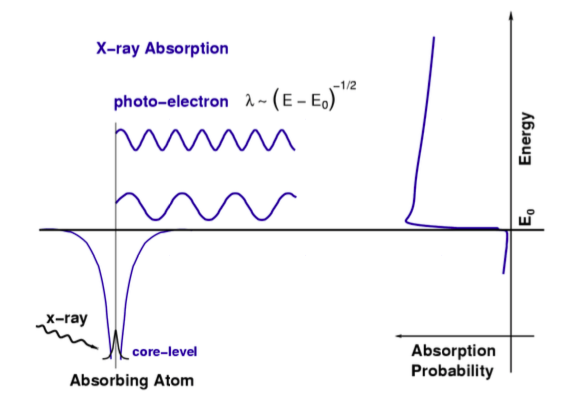
\includegraphics[width=0.8\textwidth]{../Kuvat/absorption1.png}
  \caption{The x-ray absorption through the photoelectric process is expressed visually above. When the incident photon has the energy of a tightly bound electron level, $E_0$, the absorption probability has a clear edge. The tightly bound core level is destroyed in the process and a photo-electron is created. The photo-electron travels as a wave with wave number proportional to $\sqrt{(E-E_0)}$} \cite{?}.
\end{figure}

Atom however often have a chemical environment and are not isolated. If we include one neighbouring atom into our picture, the photo-electron can now scatter from the electrons of the neighbouring atom. The scattered photo-electron can also return back to the absorbing atom. The back-scattered photo-electron can alter the absorption coefficient, since absorption coefficient depends on the available state. The back-scattered photo-electron thus causes constructive and destructive interference with the photo-electron, which is the origin of the fine-structure. This interaction with the neighbouring atom is displayed in figure \ref{fig:neighbour atom}.

\begin{figure}[h!]
  \label{fig:neighbour atom}
  \centering
  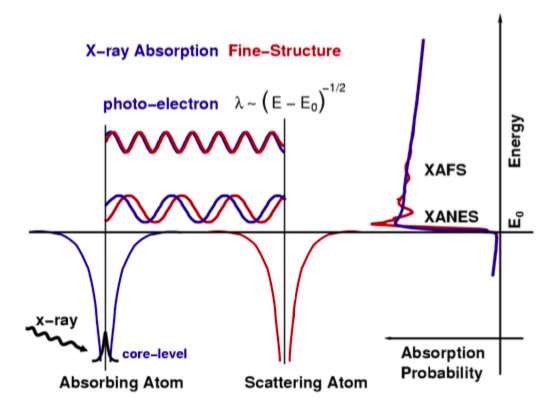
\includegraphics[width=0.8\textwidth]{../Kuvat/absorption2.png}
  \caption{something}
\end{figure}

\subsection{EXAFS}
In EXAFS the main interest are the oscillations well above the absorption edge. The EXAFS fine-structure $\chi(E)$ is defined as 
\begin{equation}\label{eq:fine-structure}
\chi(E)=\frac{\mu(E)-\mu_0(E)}{\Delta\mu_0(E_0)}
\end{equation}
where $\mu(E)$ is the measured absorption coefficient, $\mu_0(E)$ is a smooth background function describing the bare atom absorption and $\Delta\mu_0$ is the measured jump in the absorption $\mu(E)$ at the threshold energy $E_0$ as seen in figure \ref{fig:typicalxas}.   

Instead of photon energy $E$, it is common to use the wave number $k$ of the photo-electron 
\begin{equation}\label{eq:k}
k=\sqrt{\frac{2m(E-E_0)}{\hbar^2}}
\end{equation}
where $E_0$ is the absorption edge energy and $m$ is the electron mass. The main interest in EXAFS is thus the oscillations as a function of wave-number: $\chi(k)$. $\chi(k)$, often called as "the EXAFS", decays quickly with $k$. The oscillations can be emphasized by multiplying by a power of $k$.

Different near-neighbour coordination shells correspond to different frequencies observable in the oscillations of $\chi(k)$. This can be modelled by the EXAFS equation: 
\begin{equation}\label{eq:EXAFS}
\chi(k)=\sum_j\frac{N_jf_j(k)e^{-2k^2\sigma_j^2}}{kR_j^2}
\end{equation}
where $f(k)$ and $\delta(k)$ are scattering properties of the neighbouring atoms, $N$ is the number of the neighbouring atoms, $R$ is the distance of neighbouring atoms and $\sigma^2$ is disorder in the neighbour distance. This equation allows one to determine $N, R$ and $\sigma^2$, and since the scattering amplitude $f(k)$ and phase-shift $\delta(k)$ depend on the $Z$ of the neighbouring atoms, EXAFS is also sensitive to the atomic species of those neighbours.

%X-ray absorption is a transition between two quantum states. In the initial state an x-ray, a core-electron, and no photo-electron are expected, and in the final state no x-ray, a core hole and a photo-electron. With the initial and final state we can describe the $\mu(E)$ with Fermi's Golden Rule

%\begin{equation} \label{eq:Fermi}
%\mu(E) \propto |\braket{i | H | f}|^2
%\end{equation}
%where $\bra{i}$ is the initial state, and the $\ket{f}$ the final state, and $H$ is the Hamiltonian representing the interaction. The core-electron is tightly bound in the absorbing atom, so the initial state is not altered in the presence of a neighbouring atom. However the photo-electron will be able to see the neighbouring atom and thus the final state will be affected. By expanding the $\ket{f}$ into two pieces, $\ket{f_0}$ that represents the bare atom portion and the $\ket{\Delta f}$ represents the neighbouring atom, we get  


%\begin{equation}
%\ket{f}=\ket{f_0}+\ket{\Delta f} 
%\end{equation}
%which can be applied to equation \ref{eq:Fermi}
%\begin{equation}
%\mu(E)\propto |\braket{i | H | f}^2[1+\braket{i|H|\Delta f}\frac{\braket{f_0|H|i}^*}{|\braket{i|H|f_0}|}+C.C]
%\end{equation}
%where $C.C.$ stands for complex conjugate. This resembles the closely previously discussed relation between $\mu(E)$ and $\chi(E)$  
%\begin{equation}
%\mu(E)=\mu_0(E)[1+\chi(E)].
%\end{equation}

%Combining the previous equation allows us to assign $\mu_0=|\braket{i|H|f_0}|^2$ as the bare atom absorption, which depends only on the absorbing atom. We also note that the fine-structure $\chi$ can be written as
%\begin{equation}
%\chi(E)\propto\braket{i|H|\Delta f}.
%\end{equation}



\section{The XANES Section of the Spectrum}
The XANES region is much easier to measure than the EXAFS region. This is mainly due to the fact that the intensity oscillations are larger and the energy range is smaller. XANES can be done with lower concentrations and the restrictions in sample conditions are not as tight. However the XANES cannot be simply solved analytically, since the EXAFS equation breaks down at low $k$ values, mainly due to the $1/k$ term and the increase in mean-free-path at very low $k$. This however doesn't mean that we couldn't draw any conclusion from the spectra, since there is much chemical information in the XANES region. Most notably the sensitivity to oxidation number.

Typical XANES spectra can be roughly divided into few specific regions. The pre-edge, shown in figure \ref{fig:XANESfetures} as the red region, consists of small features between the Fermi energy and the threshold. The edge or the rising edge, the purple section in figure \ref{fig:XANESfetures}, is the main rising part of XANES spectra. Near-edge is the green part in figure \ref{fig:XANESfetures}. 

\begin{figure}[h!]
\label{fig:XANESfetures}
  \centering
  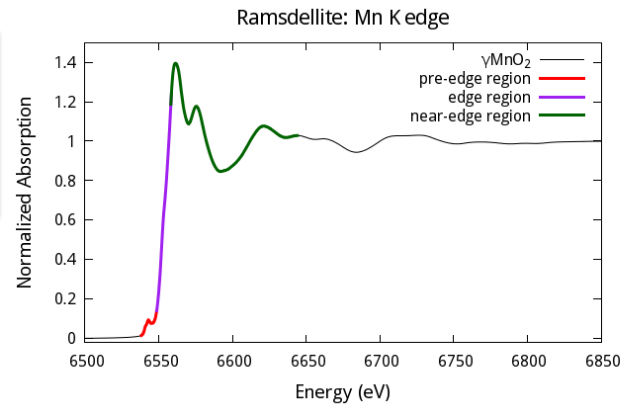
\includegraphics[width=\textwidth]{../Kuvat/XANESparts.png}
  \caption{Figure showing different features in the XANES region \cite{?}.}
\end{figure}

Qualitatively XANES can used as a "fingerprint" of the electronic structure. These "fingerprints" can be compared to known model complexes. With the "fingerprint" and known "reference" samples can be compared with principal component analysis to determine the amount of the "reference" material in the sample. 

In order to get more quantitative results one can use molecular orbital-based approach. This method works when analysing the pre-edge and the bound state transitions. By using ligand field theory one can understand the energy and and intensity distribution of the pre-edge\cite{?}. In order to get a grasp of rising edge and the near-edge, one can use multiple-scattering approach to simulate the structure. Commonly used programs are FEFF and MXAN \cite. Multiple-scattering approach can be difficult to relate back to the molecular orbital-based picture \cite{?}. 

\subsection{Multiple Scattering Events}
The x-ray excited photoelectron can be scattered by more atoms than a single one. In fact photoelectron can scattered by two or more atoms prior to returning to the absorbing atom, as seen in figure \ref{fig:ms}. The XANES region is sensitive to multiple scattering events, since the the photoelectron has a low kinetic energy and the mean free path is increased. In addition the Debye-Waller damping factor is $\exp{-k^2}$ dependent and thus negligible in the XANES region. Multiple scattering events complicates simulation of XANES, since there are more interactions and large number of multiple scattering pathways. Even though the multiple scattering events complicates simulations, they also provide a possibility to extract information about the three-dimensional structure from XANES spectra \cite{?}. Recently the simulations have become more and more accurate \cite{?}, but most of the simulations still remain qualitative.

\begin{figure}[h!]
\label{fig:ms}
  \centering
  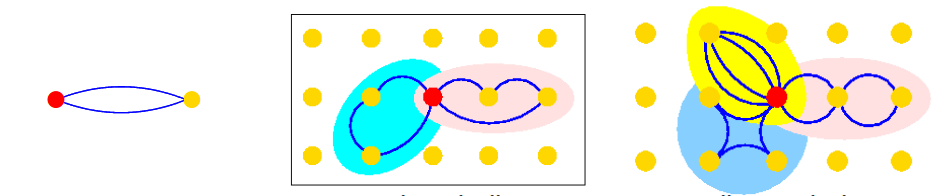
\includegraphics[width=0.4\textwidth]{../Kuvat/multiplescattering.png}
  \caption{Dashed line represents single scattering, and solid lines multiple scattering pathways. $A$ is the absorbing atom, which in this example is surrounded by two scattering atoms, $S_1$ and $S_2$ \cite{?}.}
\end{figure}

The changes in the three-dimensional structure can be seen empirically in the XANES spectra. Even small variations in structure can be seen in spectra, and for example two sites with identical EXAFS spectra can have distinct XANES spectra. Geometrical differences between sites alter the multiple scattering pathways, and this atleast partly explains the site sensitivity of XANES. The interpretation of XANES spectra has been progressing steadily, but the agreement between computational and observed spectra remains quite poor in most cases. The development of theoretical and computational model for detailed interpretation of XANES spectra remains one of the main challenges in the field.

\subsection{Oxidation Number}


The absorption edge is loosely defined. Typically it is defined as half height of the edge or as maximum of the first derivative with respect to energy. Often the definition is not as straight forward, since the edge spectra might have unresolved transitions superimposing on the rising edge. These make the definition of a unique edge energy rather troublesome. Even though defining an exact edge can be troublesome, the edge energies are useful tool for determination of oxidation state of the absorption site. The energy of an edge increases as oxidation state of the absorber increases. By using electrostatic model we can note that atoms with higher oxidation state should have higher charge, and to eject a core electron, a higher energy x-rays are needed \cite{?}. 

Alternatively we can treat the edge features as "continuum resonances" \cite{?}. A continuum resonance involves excitation of a core electron into a high-energy state, above the continuum, with a finite lifetime. Let's use the potential well between absorbing and scattering atoms as an example. As the distance between the atoms gets shorter, the energy of the continuum state increases as $1/R^2$. Higher-oxidation-state metals have shorter bond lengths this model also predicts the increase in edge energetic with increasing oxidation state. The remark of higher oxidation number increasing the edge energy is widely used in coordination chemistry.

\begin{figure}[h!]
\label{fig:FeOxidation}
  \centering
  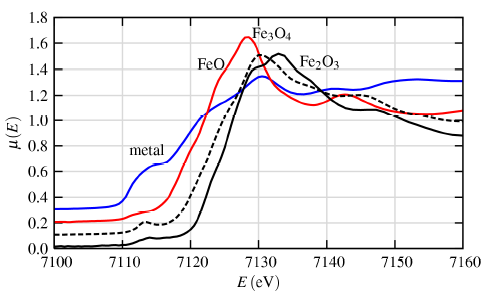
\includegraphics[width=\textwidth]{../Kuvat/FeOxidation.png}
  \caption{\ch{Fe} $K$-edge XANES spectra of metallic \ch{Fe} and some \ch{Fe} oxides. The graph clearly shows relation between oxidation state and edge energy \cite{Fundamentals}.}
\end{figure} 

The figure \ref{fig:FeOxidation} is a great example of the valance dependence of the metallic \ch{Fe} and other \ch{Fe} oxides. With good quality reference samples it is easy determine the ratios of different oxides in the sample.
       

\subsection{The Pre-edge}
In the figure \ref{fig:XANESfetures} we see a weak pre-edge peak. The pre-edge peak is caused by bound state transitions. The pre-edge is not always a simple bump in a spectra, it might have a more complicated shape, as seen in figure \ref{fig:pre-edge}. This intensity pattern is a result of multiple dependencies. The spin state, oxidation state, Ligand-Field splitting and Multiplet-effects can all affect the pattern \cite{?}. By taking intensity-weighted average energy of the pre-edge, one can notice, that it is modulated by Ligand-Field strength \cite{}. To perform this kind of analysis on the pre-edge, one needs a high quality measurement with very little noise, since the features of the pre-edge can be rather small.
\begin{figure}[h!]
  \label{fig:pre-edge}
  \centering
    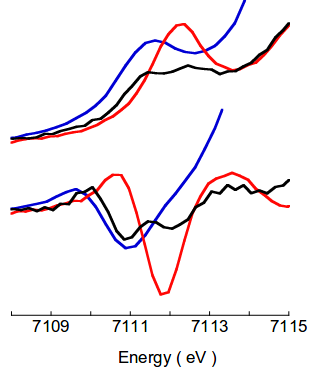
\includegraphics[width=0.6\textwidth]{../Kuvat/pre-edge.png}
  \caption{The pre-edge features of certain XANES-spectra above, and intensity-weighted average energy below \cite{?}.}
\end{figure}

 In case of K edge of a first row transition metal, the peak is caused by $1s\rightarrow 3d$ transition. The $1s\rightarrow 3d$ transition is not allowed transition according to dipole selection rule, but it is still observed due to $3d+4p$ mixing and to direct quadrupolar coupling. We can use intensity of the $1s\rightarrow 3d$ transition into our advantage to determine the geometrical structure. As the $3d+4p$ mixing improves the $1s\rightarrow 3d$ transitions increase as well, which can be used as a tool to determine bond symmetry, for example tetrahedral or octahedral \cite{?}. In some cases the bond symmetry can also be an indicator for valance \cite{?}. $1s\rightarrow 3d$ transitions have also been used in electronic band structure calculations since band structure calculations also involve multiple-scattering paths of electrons in a solid similar to XANES \cite{?}.  


Sometimes it is also possible to probe higher-lying exited states with XANES. For the first row transition series metals the $1s\rightarrow 4p$ transition is sometimes observed. The $1s\rightarrow 4p$ transition is more intense for a square-planar complexes, and weaker in case of tetrahedral complexes \cite{?}. These transitions are seen in slightly higher energies than the actual pre-edge, but below the the main edge. 
  
A complimentary approach to the metal XANES is to use Ligand XANES to study the electronic structure \cite{?}. For example in case of sulphur or chlorine ligands the metal-ligand orbital mixing (i.e. covalency) can be quantitated by this approach \cite{?}. In case of Ligand XANES we are interested in $1s\rightarrow 3p$ transition for \ch{S} and \ch{Cl}, which is allowed transition and much easier to detect, than the $1s\rightarrow 3d$ transition in case of metal XANES.  
%In case of the second row transition metals the $1s\rightarrow 4d$ transition is tricky to measure. Edge energies are higher, which decreases the core-hole lifetime, and at higher energies monochromator resolutions tend to be poor. As a result the edges are broader and the $1s\rightarrow 4d$ transition is undetectable.   

\subsection{Multi-Electron Transitions}
At higher photon energies it is possible that X-ray has enough energy to excite an extra electron into the valance band, resulting in double excitation. It is also possible, that continuum states contribute to multi-electron excitations. This multi-electron excitation is also referred to as a shake-up transition \cite{?}.

There is also other class multi-electron excitation. In this case the excitation of a core electron has the effect of converting an atom with atomic number $Z$ into an atom with atomic number $Z+1$. For example in case of $\ch{Cu}^{II}$ in the $\underline{1s}4p^I$ state, the valance electrons experience the effective nuclear charge of $\ch{Zn}^{II}$. This makes the $\underline{1s}3d^94p^1$ transition and multi-electron $\underline{1s}3d^{10}4p^1\underline{L}$ transition possible, where Ligand electron has been transferred to a lower energy \ch{Cu} 3d orbital. In this case the multi-electron transition is called the shake-down transition. The shake down transitions are often observed in photoelectron spectroscopy, but in XANES they often not taken into account. Only in case of $\ch{Cu}^II$ there is good theoretical and experimental evidence of shake-down transitions \cite{?}. However shake-down and other multi-electron transitions are likely contributing to many XANES spectra \cite{?}.   


\section{Measuring the Transmission.}\label{transmission}
Total absorption is much larger signal than the fine-structure we are interested in, which $\mu(E)$ has to be well measured. With large errors in the measurement of $\mu(E)$ the fine-structure can weaken and possibly even destroy the fine-structure.

In order to measure the absorption coefficient accurately, few components are essential. XAS is performed with an x-ray source that provides large range of wavelengths, from which a monochromator that uses Bragg's diffraction selects a particular energy. Monochromators are made from silicon and the characteristics of a monochromator can greatly influence the measurement quality. Reproducibility and stability of the monochromator along with its energy resolution are particularly important in XAS measurement. Sufficient energy resolution for XAS is $\sim 1 \si{\electronvolt}$ at $10 \si{\kilo\electronvolt}$. Over the years the production of silicon crystal has evolved and now days the stability and reproducibility are generally quite good. Another important component is the detector. A good transmission measurement of $I$ and $I_0$ is relatively easy, and even simple ion chamber is adequate.

To further increase the accuracy of the measurement the beam should be well aligned, and the sample should be homogeneous and free from pinholes. In an adequate measurement the noise levels should be $10^{-3}$.

Samples with large concentrations of the element of interest should be measured in transmission. The thickness of the sample obviously affects the transmission, so the sample should be thin enough for decent signal. From equation \ref{eq:beer} we get $x=\ln{(I/I_0)}$ for the thickness. The thickness is typically chosen so that we get $\mu x\approx2.5$ above the edge and/or $\Delta\mu(E)x\approx1$ edge step. In our case we use dilute solutions, so the sample thickness can be in the millimetre range.

When all these factors are taken into consideration, the transmission measurement is rather straightforward and one should easily obtain good quality data. 

\chapter{HelXAS}\label{setup}
\section{Setup}
We are using the X-ray absorption spectrometer, HelXAS, found in the X-ray Laboratory of University of Helsinki, to perform our measurements. The HelXAS equipment was built by the X-ray Laboratory staff. The instrument is based around three basic components: x-ray tube, monochromator and scintillator counter (detector). The monochromator crystal is placed on a motorized rail, and it can also be rotated around its vertical axis essentially to change the angle of the monochromated beam. The detector is also placed on two motorized rails to allow the movement in two dimensions. The x-ray tube is fixed in position. These components follow the so called Rowland circle geometry. Rowland circle is a Bragg reflection geometry, which allows simultaneous focusing and energy analysis of the fluorescence source. The setup is shown in figure  

\begin{figure}[h!]
  \centering
  \label{fig:setup}
  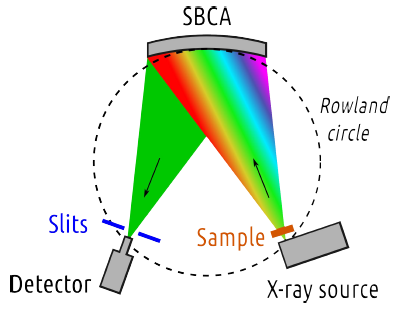
\includegraphics[width=0.8\textwidth]{../Kuvat/helxasSetup.png}
  \caption{Illustration of the measurement setup.}
\end{figure}
\subsection{X-ray Source}
HelXAS is designed to measure 3d transition metal K edges in the energy range $\approx 5-15 \si{\kilo\electronvolt}$. The x-ray source is a conventional $1.5\si{\kilo\watt}$ fine focus diffraction glass tube with a \ch{Ag} target. \ch{Ag} has characteristic lines above $20\si{\kilo\electronvolt}$ \cite{}, which extends the Bremsstrahlung region up to \ch{Mo} K edge in the periodic table. The source is suitable for $3d$ transition metal K edge and $5d$ L edge spectroscopy. 



      
\subsection{Monochromators}
The X-rays spectra produced by the X-ray tube is polychromatic and is thus not very useful for our purpose to vary the energy in a small energy band. To make the x-ray beam more useful we use a monochromator crystal. The crystal is used for point-to-point scanning, where a small energy bandwidth ($<5\si{\electronvolt}$) satisfies Bragg's diffraction condition over the whole crystal area and is focused on the detector \cite{Analyzer crystal}. The Bragg's diffraction condition 
\begin{equation} \label{eq:bragg}
2d_{hkl}\sin\theta_b=n\lambda,
\end{equation}
where $d_{hkl}$ is the distance between atoms in a lattice, $n$ is an integer, $\theta_b$ theta the angle between incident beam and diffracted beam and $\lambda$ is the wavelength of the diffracted beam. The distance $d_{hkl}$ is proportional to the miller indices, and by selecting the right crystal orientation we can also selected the wanted energy bandwidth in a point-to-point measurement. The wavelength is related to energy by 
\begin{equation}
\lambda=\frac{hc}{E},
\end{equation} 
where $h$ is Planck's constant and $c$ speed of light in a vacuum. 

For our measurement we use an analyzer crystal with miller indices $hkl=[3,5,1]$, which allows us to scan the around the k-absorption edge of \ch{Fe} at $E=7.1 \si{\kilo\electronvolt}$, by varying the angle $\theta$.

The analyser crystal is spherically bent to focus the beam to the detector. Our setup uses crystals with $0.5 \si{\metre}$ bending radius. Spherical bending however causes strain fields in the monochromator, which can alter energy resolution. Strain field effect is addressed by cutting the surface in $15 \si{\milli\metre}$ wide strips. The typical energy resolution of our analysers is $\gtrsim 1 \si{\electronvolt}$. Our strip-bent spherically bent crystal analysers (SBCA) are provided by ESRF Crystal Analyser Laboratory.        

\subsection{Detectors}
HelXAS can be operated in transmission, fluorescence and imaging modes. The data can also be acquired with multiple detectors. In our case we are using the transmission mode, in which we use a Scintillator detector with a single channel analyser. The setup uses doped \ch{NaI} crystal, which converts the x-ray photons to low energy photons, which are converted to a cascade of electrons. These pulses are collected and transformed into voltage pulses. Pulses are proportional to photon energy, but the energy resolution is poor.

The detector has a finite response time to incident photons, known as dead time $\tau$. During that time the detector cannot count other photons. For sufficiently small dead time we can use the following correction

\begin{equation} \label{eq:deadtime}
N_{correct}\approx\frac{N}{1-\frac{\tau}{T}N},
\end{equation}
where $N$ is the number of counted pulses and $T$ is the time in which they were acquired. Dead time of our detector is $\tau=2.8 \si{\milli\second}$.

\subsection{Motors and movements}
Movements of the motors follow the Rowland circle geometry. The setup has three motorized linear translational stages, one motorized goniometer and one passive rotational stage with telescopic with steering bar. 3D model of the components is displayed in figure \ref{fig:cad}. 

\begin{figure}[h!]
  \label{fig:cad}
  \centering
  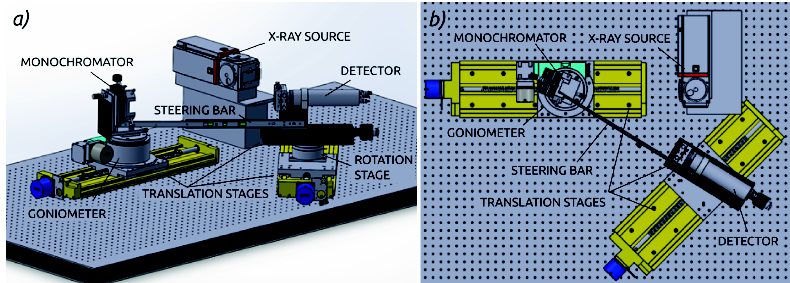
\includegraphics[width=\textwidth]{../Kuvat/cad_setup.png}
  \caption{3D model of the HelXAS setup.}
\end{figure} 

The monochromator crystal is installed on top of a Huber goniometer, which controls the Bragg's angle $\theta_B$. The crystal goniometer installation is placed on a linear stage, which controls the distance between source and monochoromator noted as $\rho$. The $\rho$ is related to $\theta_B$ as $\rho = R_bsin\theta_B$, where $R_b$ is the bending radius of monochromator crystal.  

Motors and data acquisition is run on SPEC version 6 by Certified Scientific Software.   

\subsection{Preparations for Anaerobic Samples}
For the anaerobic samples we had to design a new sample environment. In our design the sample is placed between two $0.1 \si{\milli\metre}$ kapton foils, and sealed with $1 \si{\milli\metre}$ thick o-ring. This setup is compressed by two aluminium plates and eight screws. The window on the aluminium plates has a diameter of $10 \si{\milli\metre}$, and there are 8 slots for samples. The design is show in figure \ref{fig:n�ytteenvaihtaja}.

\begin{figure}[h!]
  \label{fig:n�ytteenvaihtaja}
  \centering
  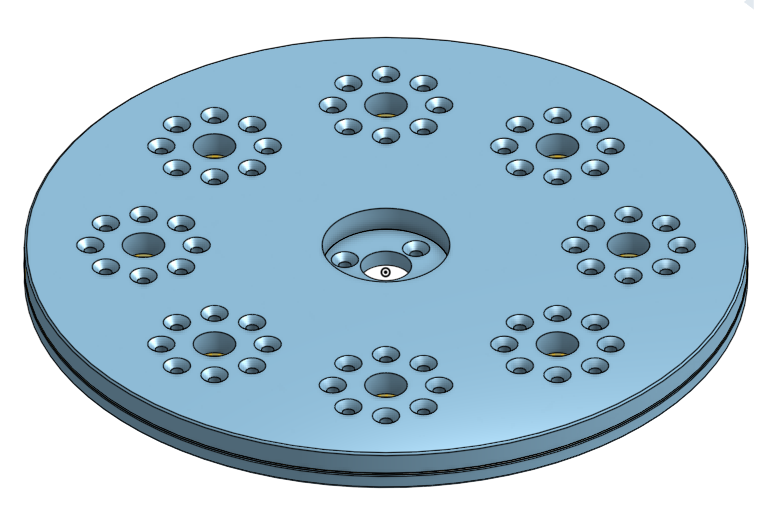
\includegraphics[width=0.8\textwidth]{../Kuvat/vaihtaja.png}
  \caption{The design of the anaerobic chambers.}
\end{figure}
The sample plate is motorized, which allows us to automate the measurements.

\subsection{Background Noise}
When doing the measurement, the background noise is always present. Background noise is caused by elastic scattering, fluorescence, etc. Since the $\mu x$ is obtained from a logarithm, it is highly non-linear, and thus sensitive to background noise. 

The background noise can be taken into account by measuring it by moving the detector away from the direct beam. The accuracy of background measurement can be improved by measuring the background from both sides of the beam and taking the mean. The background is slowly varying, so in order to avoid statistical noise, a low order polynomial is fitted and the fit is removed from the signal.    

\subsection{Measurement Procedure}
First we measure the direct beam $I_0$ and the transmitted beam $I$ and their backgrounds $I_{0,bg}$ and $I_{bg}$. Then we apply the dead time correction from equation \ref{eq:deadtime}. Next we fit low order polynomials $y$ and $y_0$ to the backgrounds $I_{0,bg}$ and $I_{bg}$. Finally we compute the $\mu x$ from equation

\begin{equation} \label{eq:mux}
\mu  x=\ln\frac{I_0-y_0}{I-y}.
\end{equation}


\chapter{Sample Preparation}\label{preparation}
\section{Reference Samples}\label{ref}
In order to estimate the chemical state of our system, we acquired a set of reference samples of some well known iron compounds. These samples can be used as a fingerprint for each compound and allow us keep track of the chemical state of our soil samples. In all of our  measurements we used $0.01\si{\milli\metre}$ iron foil to keep track of our energy calibration. 
\section{Samples}\label{samples}
\subsection{Soil Samples}
The soil we received was obtained from five different locations. The soil was weighted by using a scale with an accuracy of $10^{-4} \si{gram}$. The soil was then mixed with farina in approximately 1:4 concentration. After mixing we added some ethanol and ground using a mortar until the ethanol was evaporated. The result was a fine mix with a uniformly small particles. The mix was then placed in a M5 washer and was sealed with Scotch tape. From the five different soils we made two samples of each.  
\subsection{Jellys}
The measurement of wet samples turned out to be trickier than expected. When the sample was placed in front of the X-ray tube, the bremsstrahlung caused by the x-ray and sample atom interaction, broke the bonds in the water molecules. The broken water molecules released \ch{O}-radicals, which interacted with our samples and after few ours all the water in the sample was gone, and the chemical state of the sample was altered.

Second problem we encountered was the sample homogeneity. When the soil is mixed with water, it tends to sediment. The sedimentation causes soil to accumulate at the bottom of the sample environment. Also when the sample is rotated, the smaller particles move faster and larger particles/clusters may stay still. Now when if place the sample in front of the detector and scan the energy range by changing the angle $\theta$, we might hit just the water or the soil with different thickness or particle size. 

In order to tackle the problems stated above we decided to gel our samples with agar. We took the water where the samples were mixed in, and added approximately $1-0.5wt\%$ of agar. The water was then heated to boiling and mixed all the time with magnetic stirrer. Heating was turned off when the water reached boiling temperature and the sediment was mixed with water after the water reached approximately $60\si{celcius}$. The mix was then quickly placed in the sample environment and cooled in a fridge. This method allowed us to make homogeneous samples to be placed in front of the detector. 

We tested the optimal water/soil ratio for our samples by mixing soil and water in ratios 1:4, 1:8 and 1:16. We then measured the absorption spectra of these mixes and the results are shown in figure \ref{fig:jellytest}.
\begin{figure}[h!]
   \label{fig:jellytest}
   \centering
   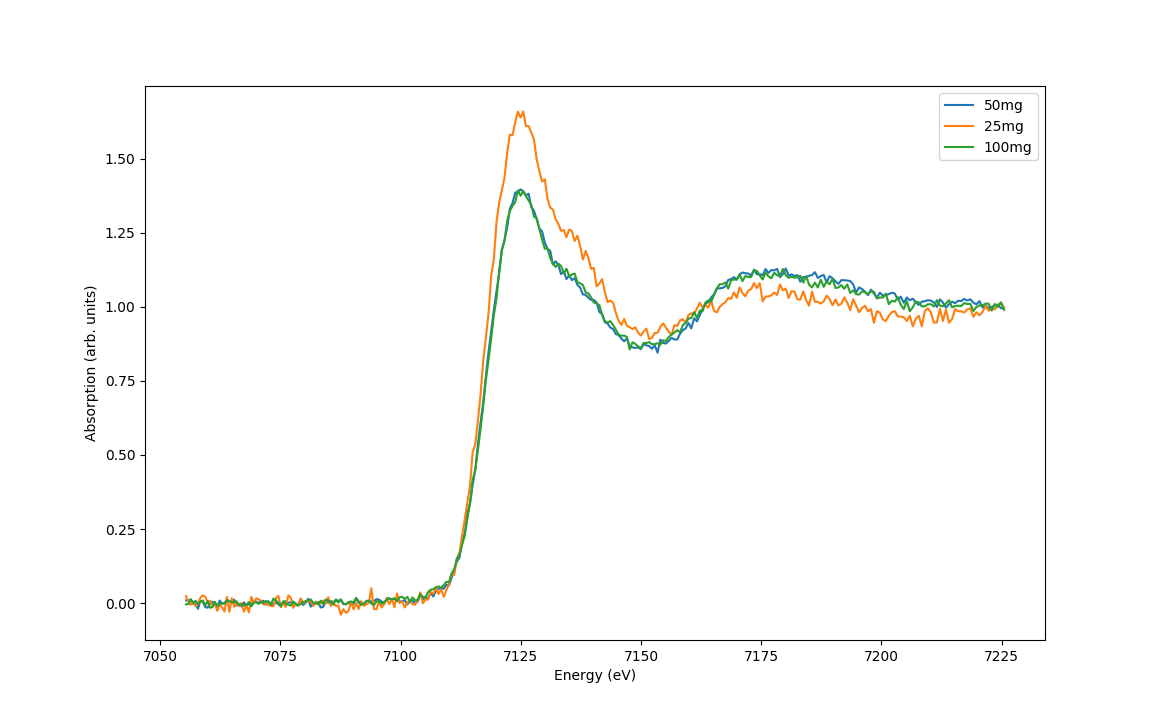
\includegraphics[width=\textwidth]{../Kuvat/JellyTest.png}
   \caption{The x-ray absorption spectra different gel mixes.}
\end{figure}
As a result for this test we concluded that we need high enough soil/water concentration to make the normalization of our spectra easier. 
\subsection{Anaerobic Jellys}
The sample preparation of anaerobic wet samples was rather similar to the preparation of our normal wet samples. The major difference was that the sample preparation was done in \ch{N2} atmosphere. The \ch{N2} atmosphere was pressurised, which made  weighing the agar rather complicated task. With most of the samples the $wt\%$ of agar was not accurate, and the amount of agar had to be estimated with approximately. The temperature in the anaerobic chamber was circulating around $30^\circ$C so we used ice and copper rods to cool the sample instead of fridge. 

Even with these constrains the sample preparation was rather straight forward and we managed to produce smooth homogeneous jelly. The samples endured the measurement and the black color on samples with \ch{C} treatment lasted until the sample environment was opened after the measurement.     

\subsection{The Effects of Agar}
In order to eliminate the radiation damage in water molecules, we decided to turn the water into a gel. This also helped us to achieve proper sample uniformity as the soil particles were "frozen" in place in the gel. The agar we used was powder for bacteriology from WVR chemicals \cite{?}. Our Agar had a melting point at $90\si{\celsius}$ and gelling point at $30-40\si{\celsius}$. This meant that we didn't need to boil our water, and when we mixed the water with soil, the temperature of the soil never increased over $50\si{\celsius}$. The changes in \ch{Fe} chemistry happen mainly through redox reactions \cite{?}, and since we only heat the sample for a relatively short time period to a modest level, we can expect that the heating won't cause any changes in the chemical state. 

As for the added agar, as it turns into a gel, it forms a double helical structure. By joining double helices, three-dimensional structure framework is formed, which holds water molecules within interstices of the framework \cite{}. Agar gel is rather stable under normal laboratory conditions. Exposure to extended periods of high temperatures and pHs lower than 6.0. These conditions can be easily avoided during our experiments. The main concern is that agar-gel is fertile media for bacteria, and in room temperatures we might see growth of micro-organisms \cite{?}. However we are able to perform our measurement within $10-14 \si{\hour}$ after the gel formation, and during that time period, the bacteria growth should still be relatively minimal. Typically visible bacteria growth is seen after 2-3 days \cite{?}.
\chapter{Results and Analysis}\label{tulokset}
\section{Analysis}
\subsection{Data Reduction}
The measured data is represents the incoming photons per measurement time in each angle step. In order to gain access to the absorption coefficient as a function of energy, we use the following steps:
\begin{enumerate}
\item The measured intensities are converted to $\mu(E)$, by using the .
\item A smooth line is fitted to the pre-edge region of the spectrum and then subtracted from the $\mu(E)$ in order to get rid of the instrumental background and absorption from other edges.
\item The threshold energy $E_0$ is identified as the maximum derivative of $\mu(E)$.
\item $\mu(E)$ is normalized from 0 to 1, so that it represents the absorption of 1 x-ray.
\end{enumerate}
\subsection{Curve fitting}
To approximate how much of a certain component was formed during the incubations, we needed to compare the result with the reference samples. Since we are comparing the initial state with a final state, in which we expect a new component, we can try to match the final state by performing a least squares fit. The least squares method minimizes the summed square of residuals to obtain the coefficient estimates. The method requires similar data grid. 

\section{Measurement results}
\subsection{Dry Soil Samples}
All the soil samples had a relatively similar spectra, as seen in the figure \ref{fig:drySoil}. The samples were collected from similar height from the sea level, so the their geological age should be relatively similar. With similar geological ages the chemical state of \ch{Fe} is expected to be similar between the samples. 
\begin{figure}[h!]
  \label{fig:drySoil}
  \centering
    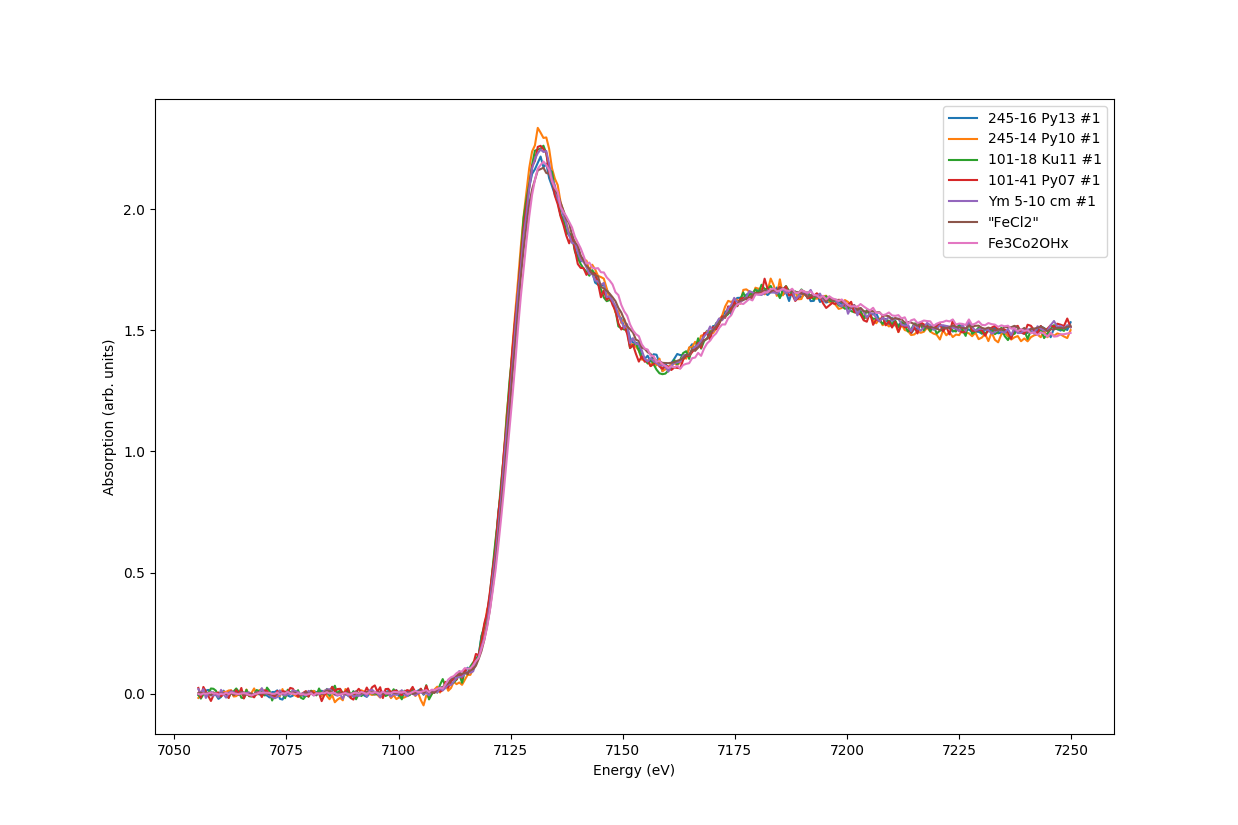
\includegraphics[width=\textwidth]{../Kuvat/Dry_Soil_Samples1.png}
  \caption{The spectra of dry soils.}
\end{figure}

Our measurement of dry soil samples produced the expected results and the spectres were very similar with different iron hydroxides. Iron hydroxides, for example ferryhydrate and goethite, have very similar spectres with each other, so with XANES it is difficult to evaluate the exact chemical state. However we can state that the iron in the samples is mainly as \ch{Fe}(III) hydroxides. The spectra might consist of multiple different \ch{Fe} hydroxides and in order to fully obtain knowledge of the components, some other characterisation technique should be used. We can use this result as a fingerprint of the initial chemical state of our system.  

We also made another sample from each of the soils to test the homogeneity of our soils. The results are shown in figure \ref{fig:dryHomogeneity}, and  as clearly visible, the soil are very homogeneous. 

\begin{figure}[h!]
  \label{fig:dryHomogenity}
  \centering
    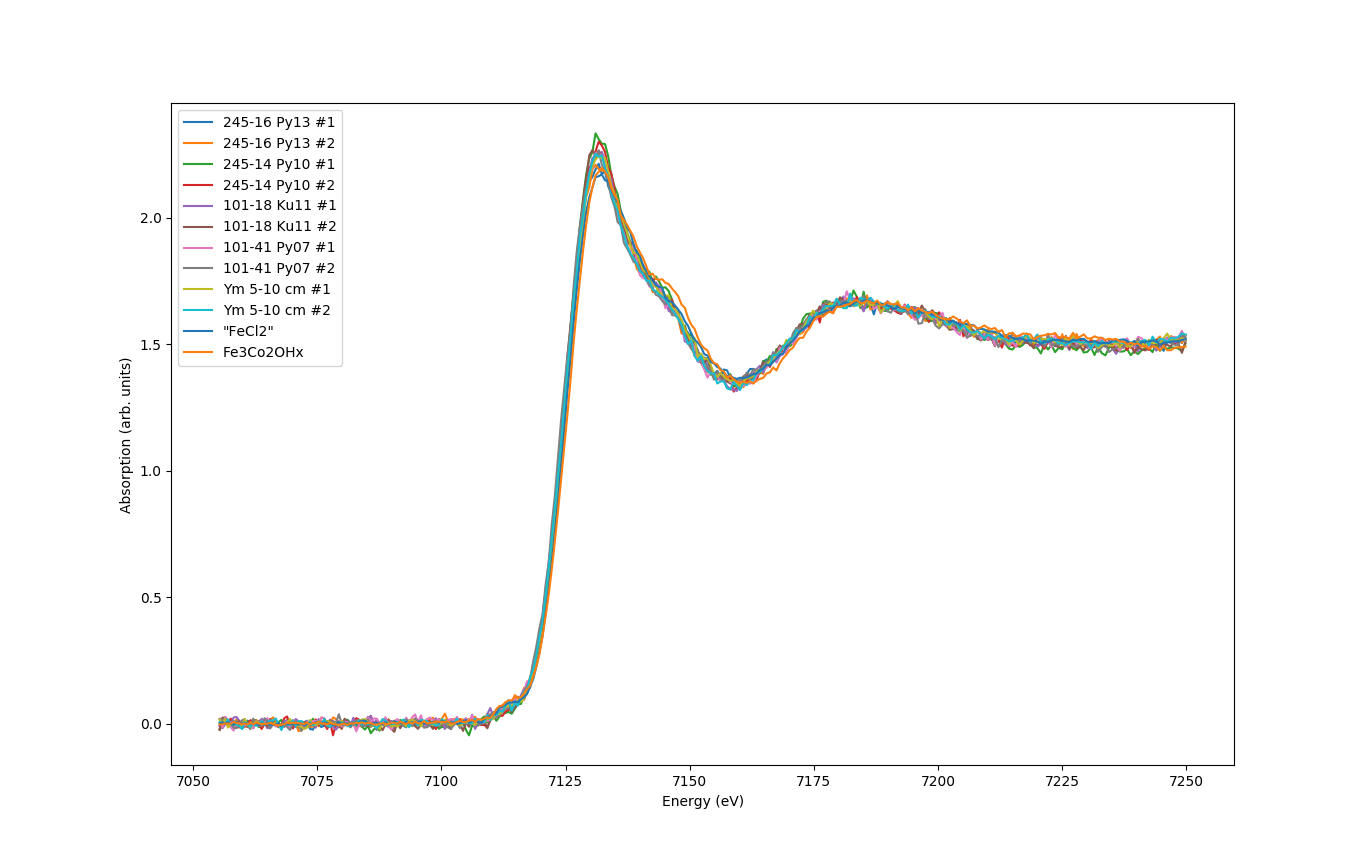
\includegraphics[width=\textwidth]{../Kuvat/dry_soil_samples_all.png}
  \caption{The spectra of all dry soils. The samples of the same soil are clearly homogeneous with each other. }
\end{figure}

\subsection{Wet Samples After 24 Hours}
The soils were then placed in glass bottles for incubations. Sea water was added and the bottles were placed in a cold and dark environment. The samples were collected from these bottles after the first 24 hours, and then made into a gel.
 
With the added water the measurement time was reduced. This caused more noise in the spectra. With the added water we expect the chemical state to remain the same with the dry samples, since the mineralization process takes several weeks to take place. The results from the measurement is shown in figures \ref{fig:wetsoil}, \ref{fig:wetsoilC} and \ref{fig:wetsoil_others}.

\begin{figure}[h!]
  \label{fig:wetsoil}
  \centering
     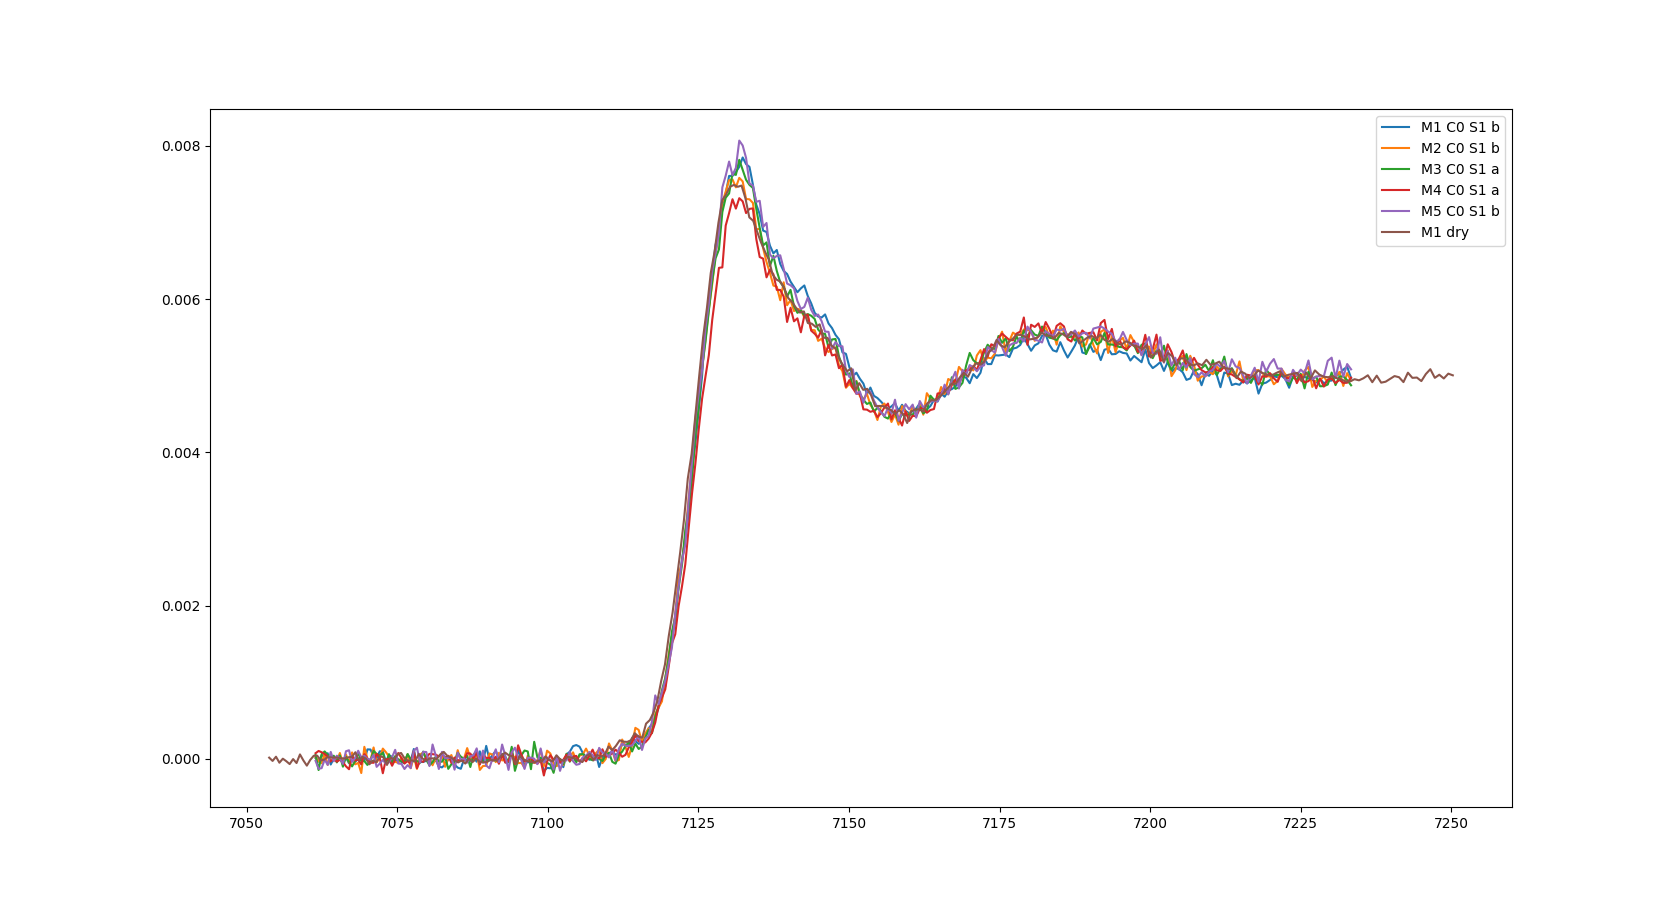
\includegraphics[width=\textwidth]{../Kuvat/Sulfideja/wet_noC.png}
  \caption{The spectra of wet samples with no added \ch{C} after 24 hours of incubation.}
\end{figure}

\begin{figure}[h!]
  \label{fig:wetsoilC}
  \centering
     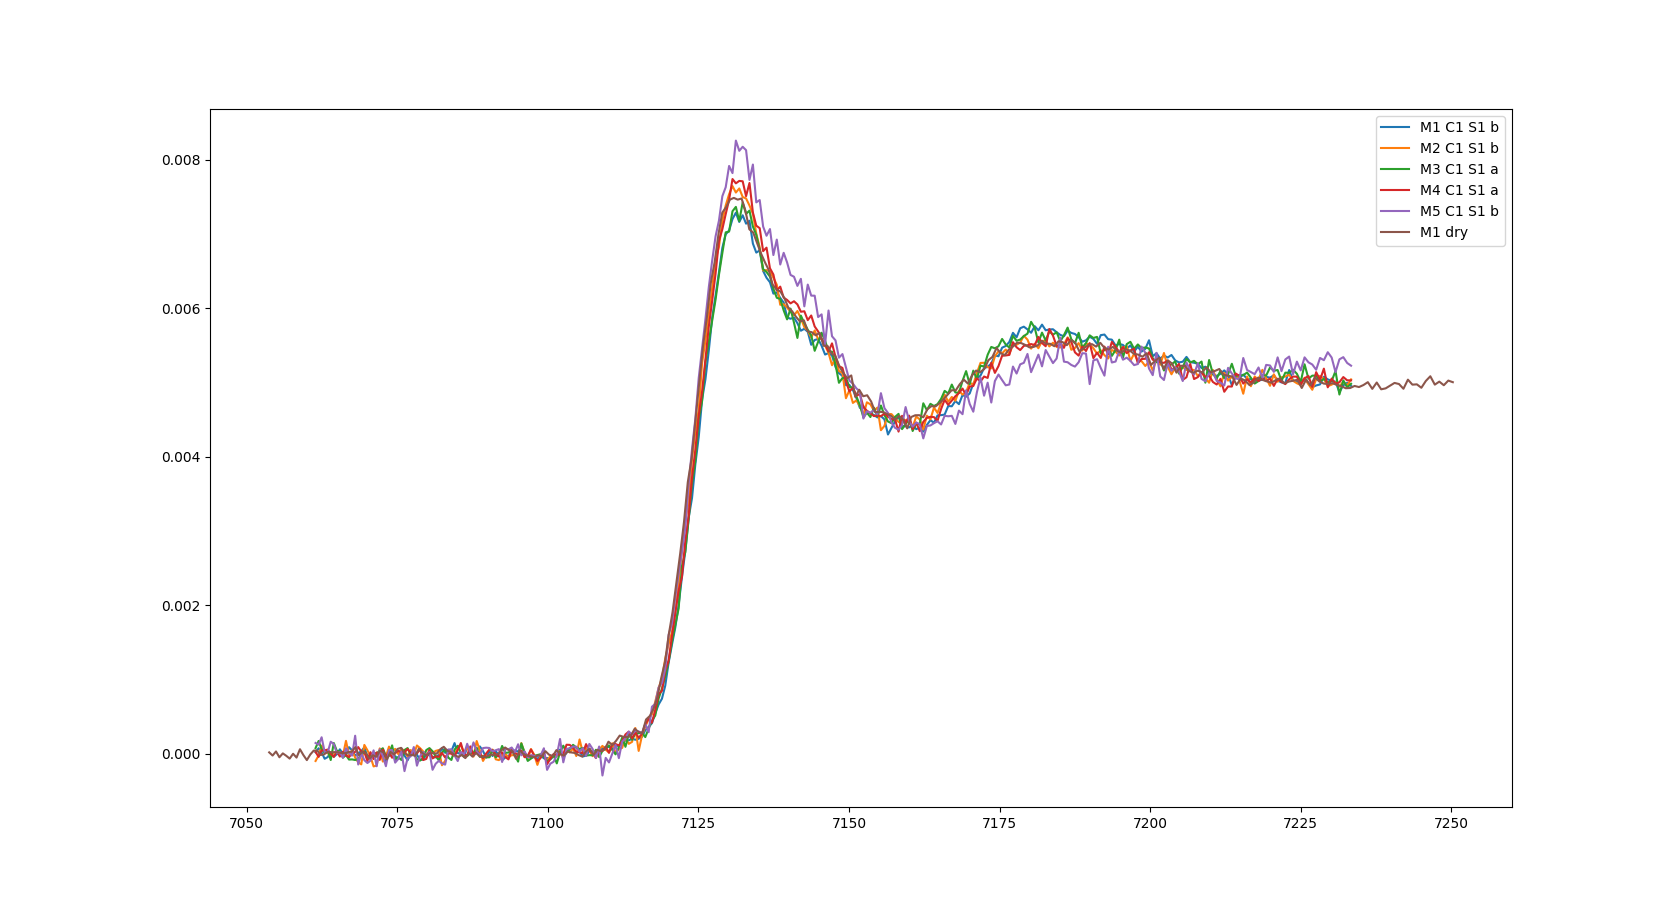
\includegraphics[width=\textwidth]{../Kuvat/Sulfideja/wetC.png}
  \caption{The spectra of wet samples with added \ch{C} after 24 hours of incubation.}
\end{figure}

\begin{figure}[h!]
  \label{fig:wetsoil_others}
  \centering
     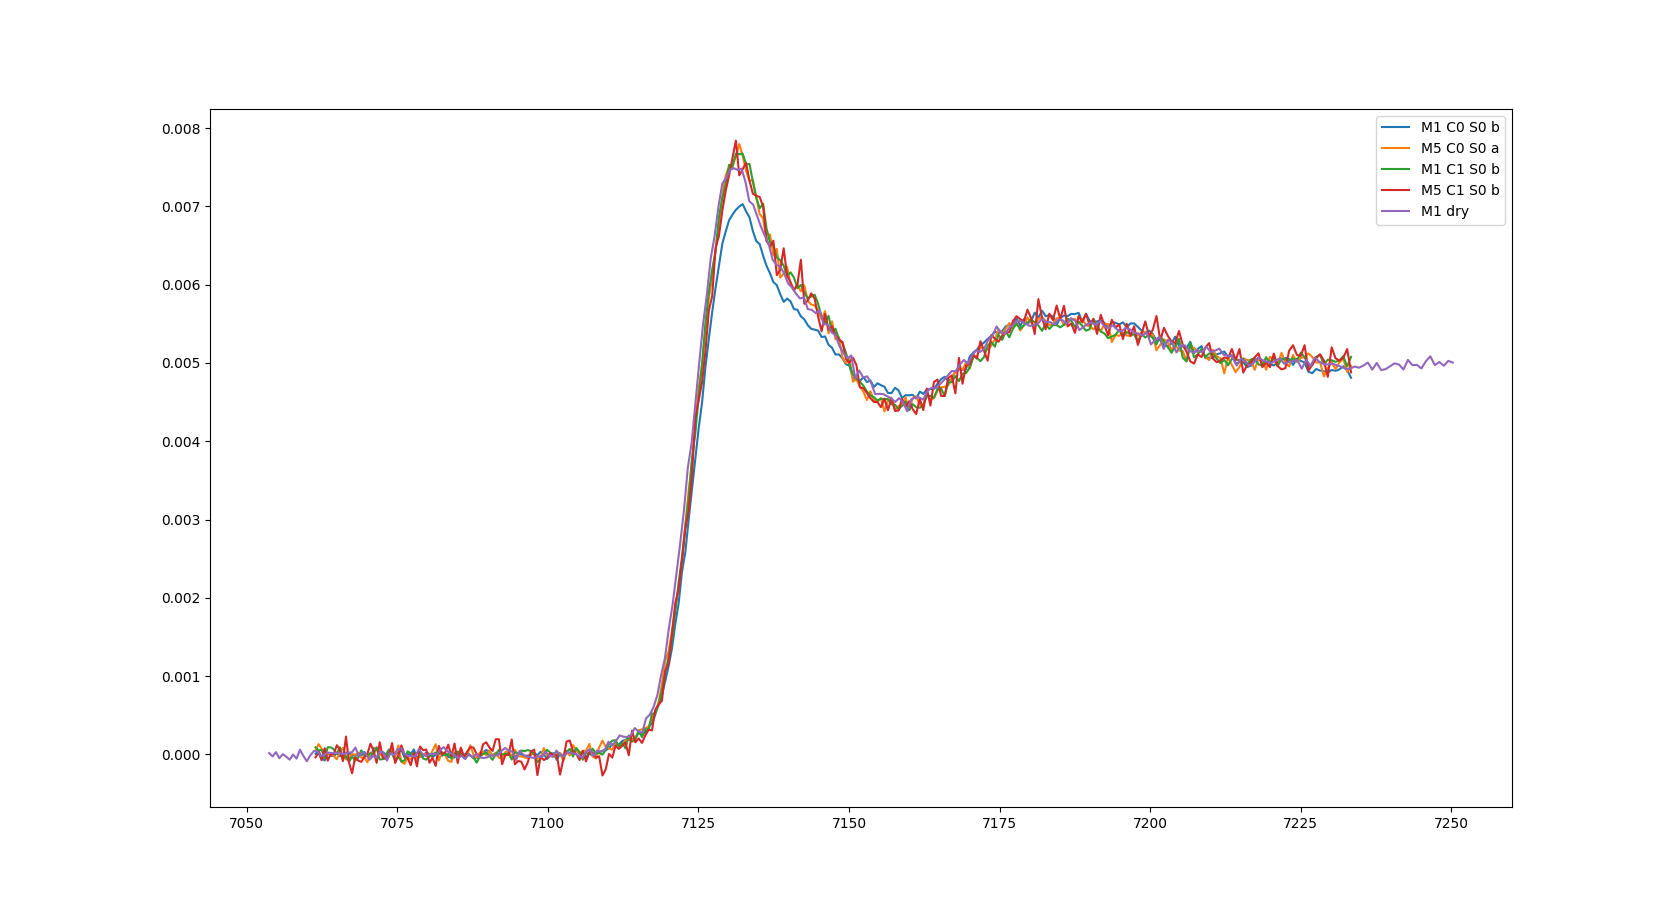
\includegraphics[width=\textwidth]{../Kuvat/Sulfideja/wetOthers.png}
  \caption{The spectra of wet samples with no added sulphides.}
\end{figure}

The chemical state seems to remain the same in all of our measurements. Two of the sample seem to have, M1C0S0b and M5C1S1b, have slightly different height in the white line region. This is propably caused by small water/soil ratio in the sample, which we discussed in the sample preparation section. The peaks, valleys and other spectral features seem to happen at similar energies compared to other samples, so the chemical state can be expected to remain the same as in the other samples. We collected our samples from larger bottles, and some of them had very small amounts of water or soil, which made the sample preparation more difficult. In the next sample taking we addressed this issue by taking larger amounts of both soil and water from the larger bottles.   

\subsection{Anaerobic Wet Samples}
We improved our measurement by splitting it into three parts. In the first 75 measurement points we used 1 second measurement time, in the next 135 measurement points 15 seconds and in the last 90 points again 1 second. This allowed us to get better quality data from the sections where we see the largest changes in the spectra in case of altered chemical state.
\subsubsection{Samples with no added \ch{C}}
In case with no added \ch{C} the samples were stored in $5\si{\celsius}$ in a dark room for two months. After two months the samples looked visually the same as after two days. XAS results however revealed an altered chemical state. The measurement results are shown in figures \ref{fig:M5_noC},. Our results showed that no sulphides were formed and no  \ch{Fe2O3} were formed either. It is clear that there is no shift in the rising edge, and thus the oxidation state has remained the same. 
\begin{figure}[h!]
  \label{fig:M1_noC}
  \centering
    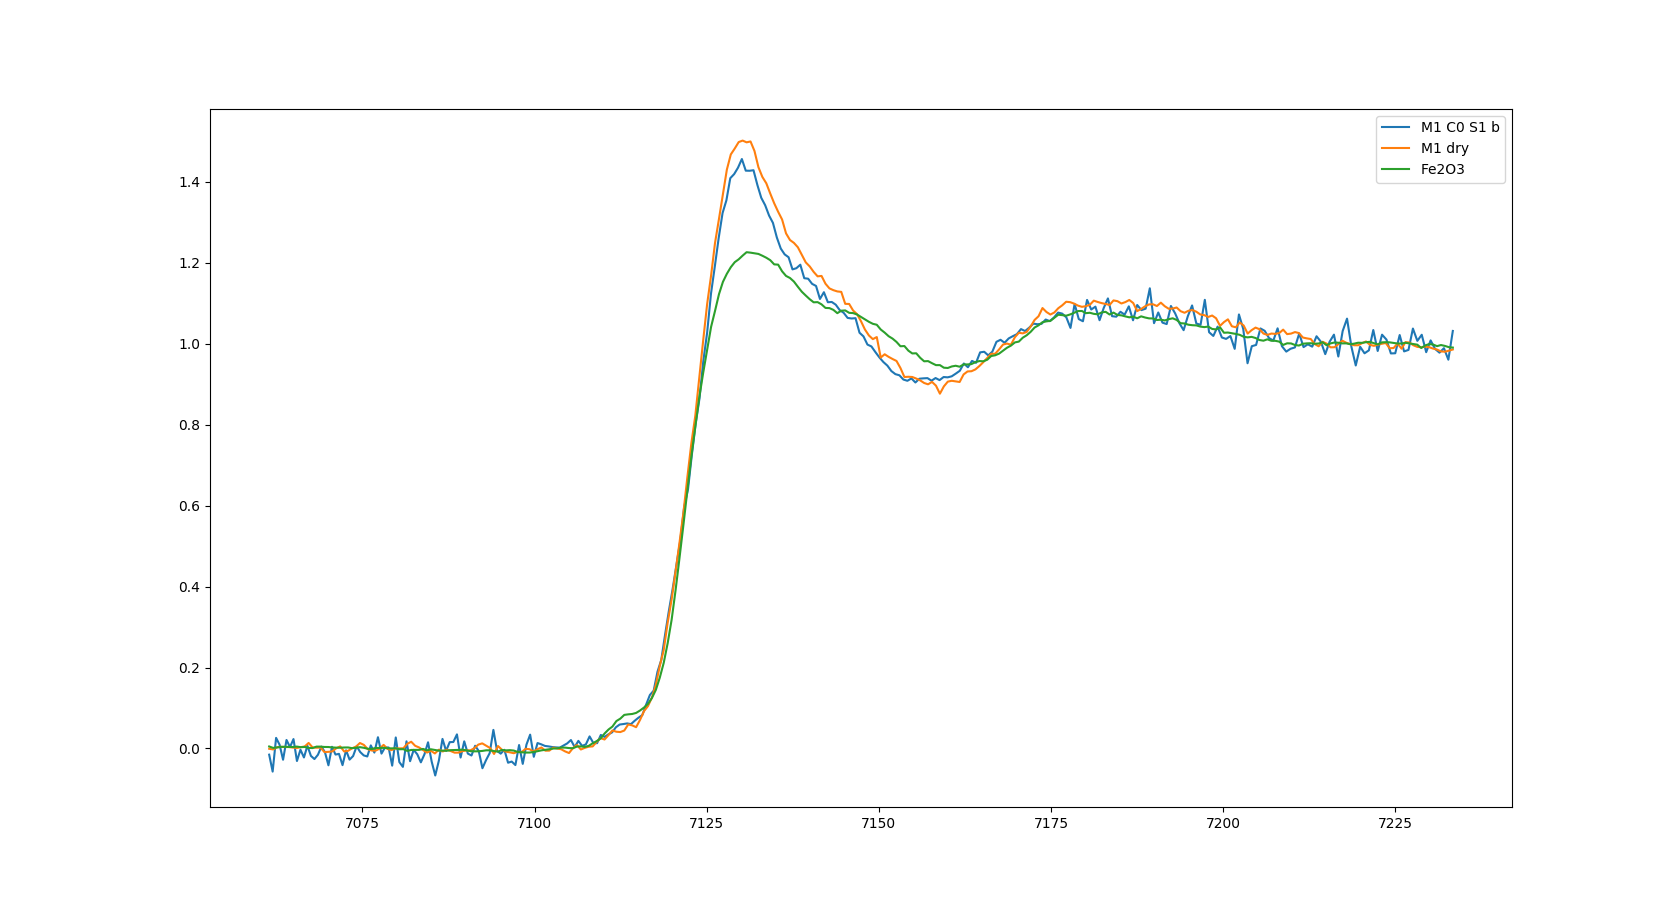
\includegraphics[width=0.9\textwidth]{../Kuvat/Sulfideja/M1_Fe2O3.png}
  \caption{M1 soil with no added \ch{C} after two months of incubation. The results are compared to the dry sample and \ch{Fe2O3} reference sample.}
\end{figure}

\begin{figure}[h!]
  \label{fig:M2_noC}
  \centering
    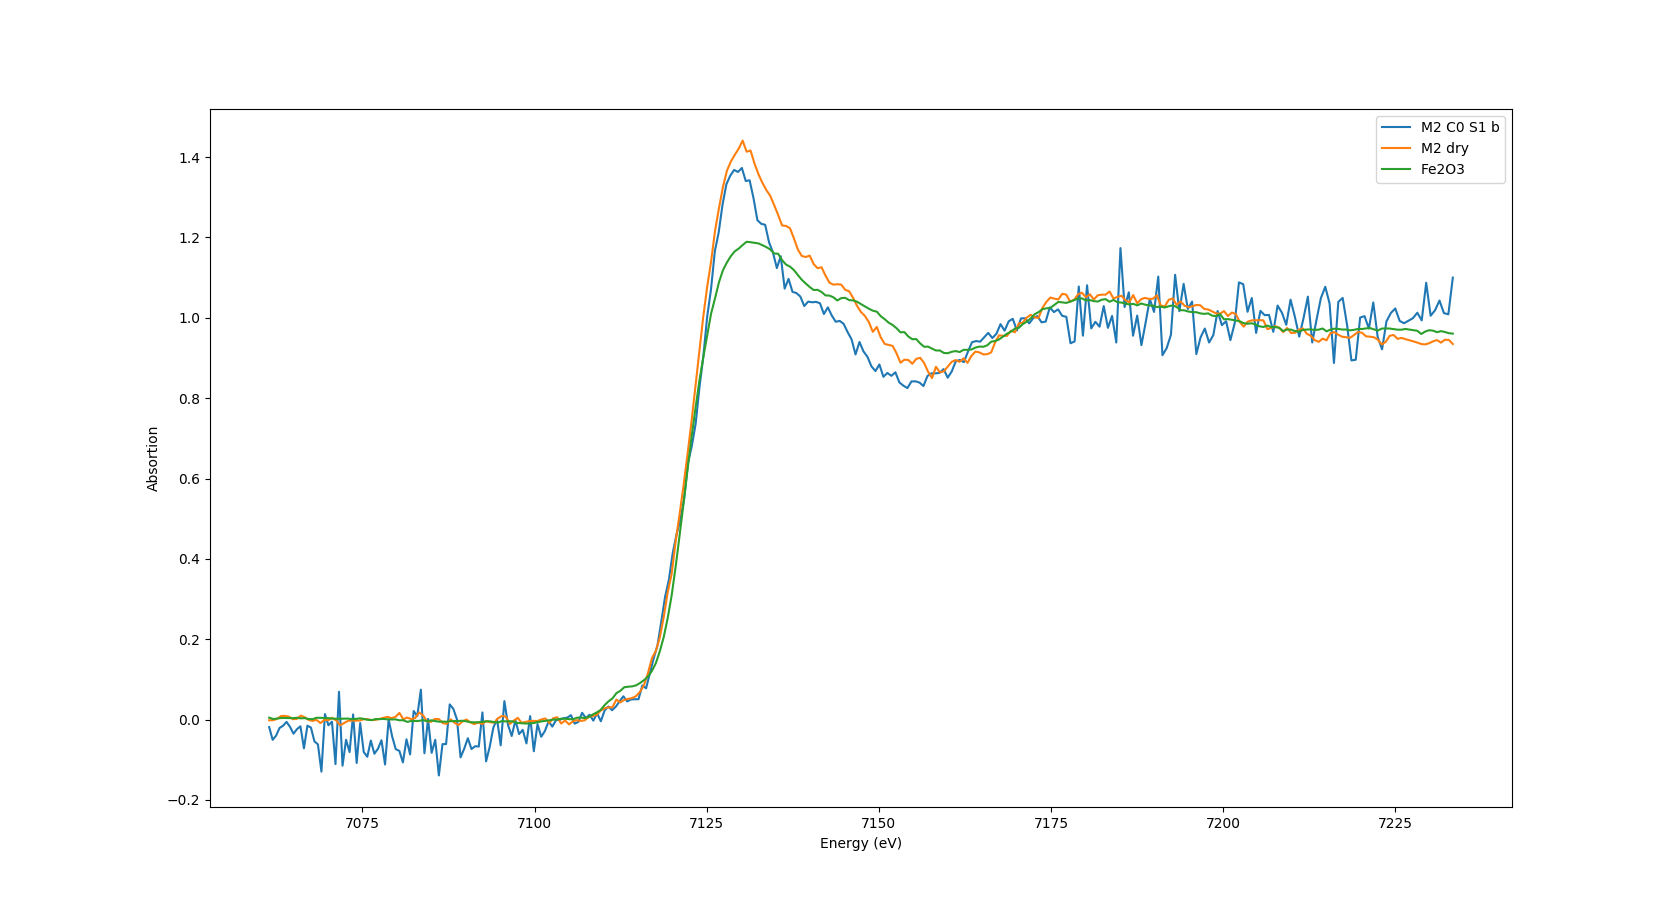
\includegraphics[width=0.9\textwidth]{../Kuvat/Sulfideja/M2_Fe2O3.png}
  \caption{M2 soil with no added \ch{C} after two months of incubation. The results are compared to the dry sample and \ch{Fe2O3} reference sample.}
\end{figure}

\begin{figure}[h!]
  \label{fig:M3_noC}
  \centering
    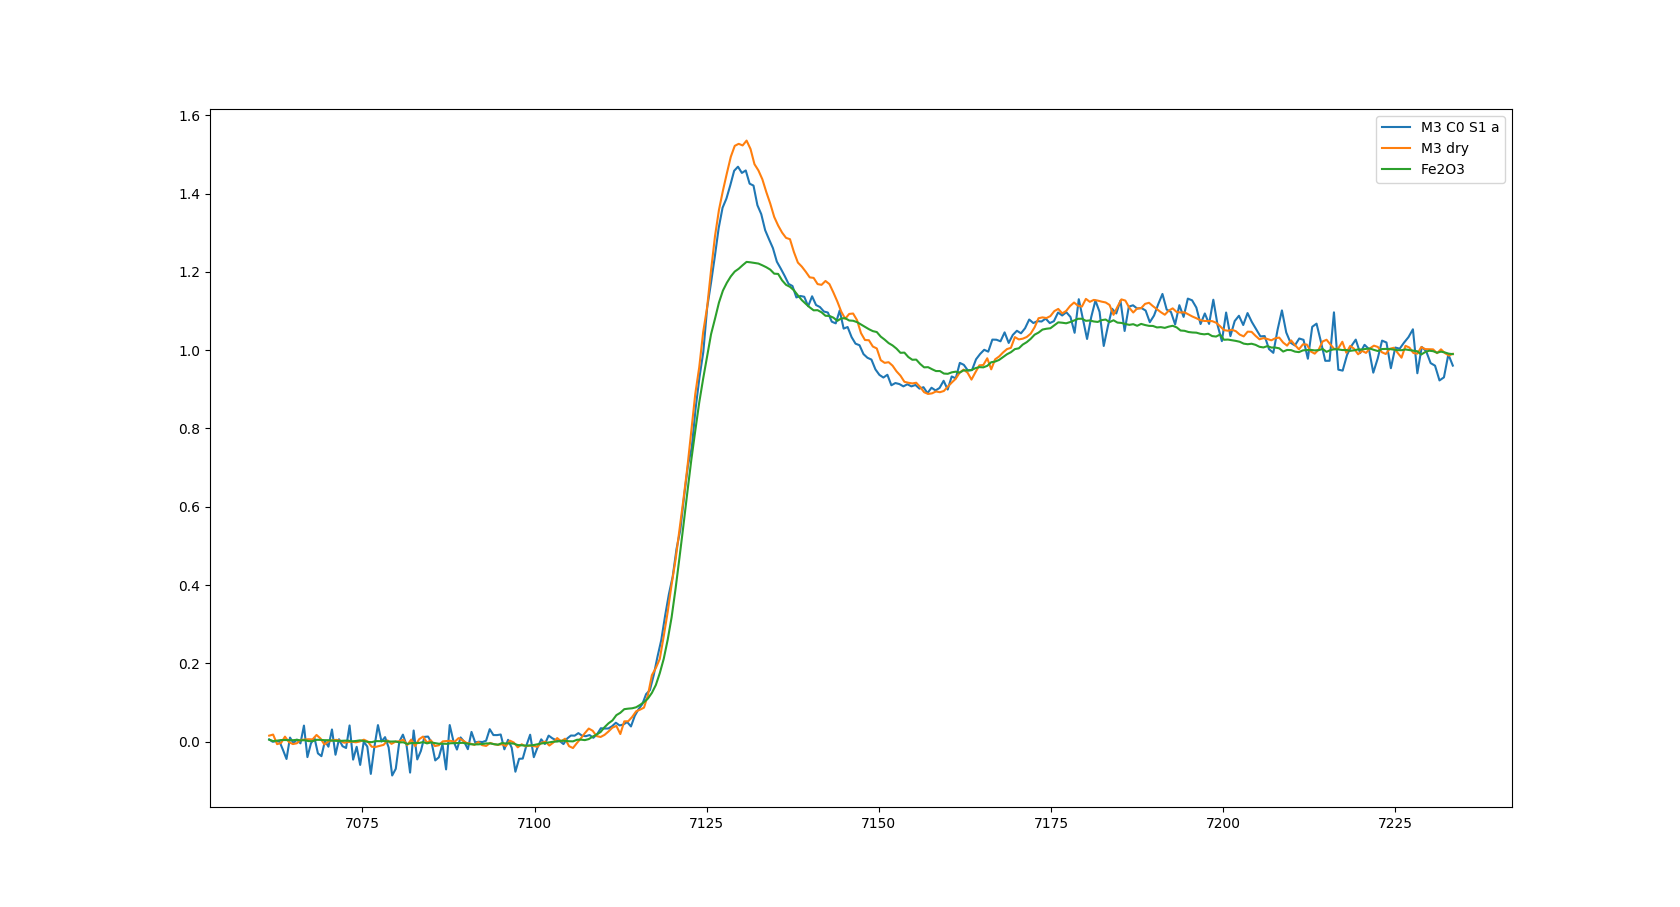
\includegraphics[width=0.9\textwidth]{../Kuvat/Sulfideja/M3_Fe2O3.png}
  \caption{M3 soil with no added \ch{C} after two months of incubation. The results are compared to the dry sample and \ch{Fe2O3} reference sample.}
\end{figure}

\begin{figure}[h!]
  \label{fig:M4_noC}
  \centering
    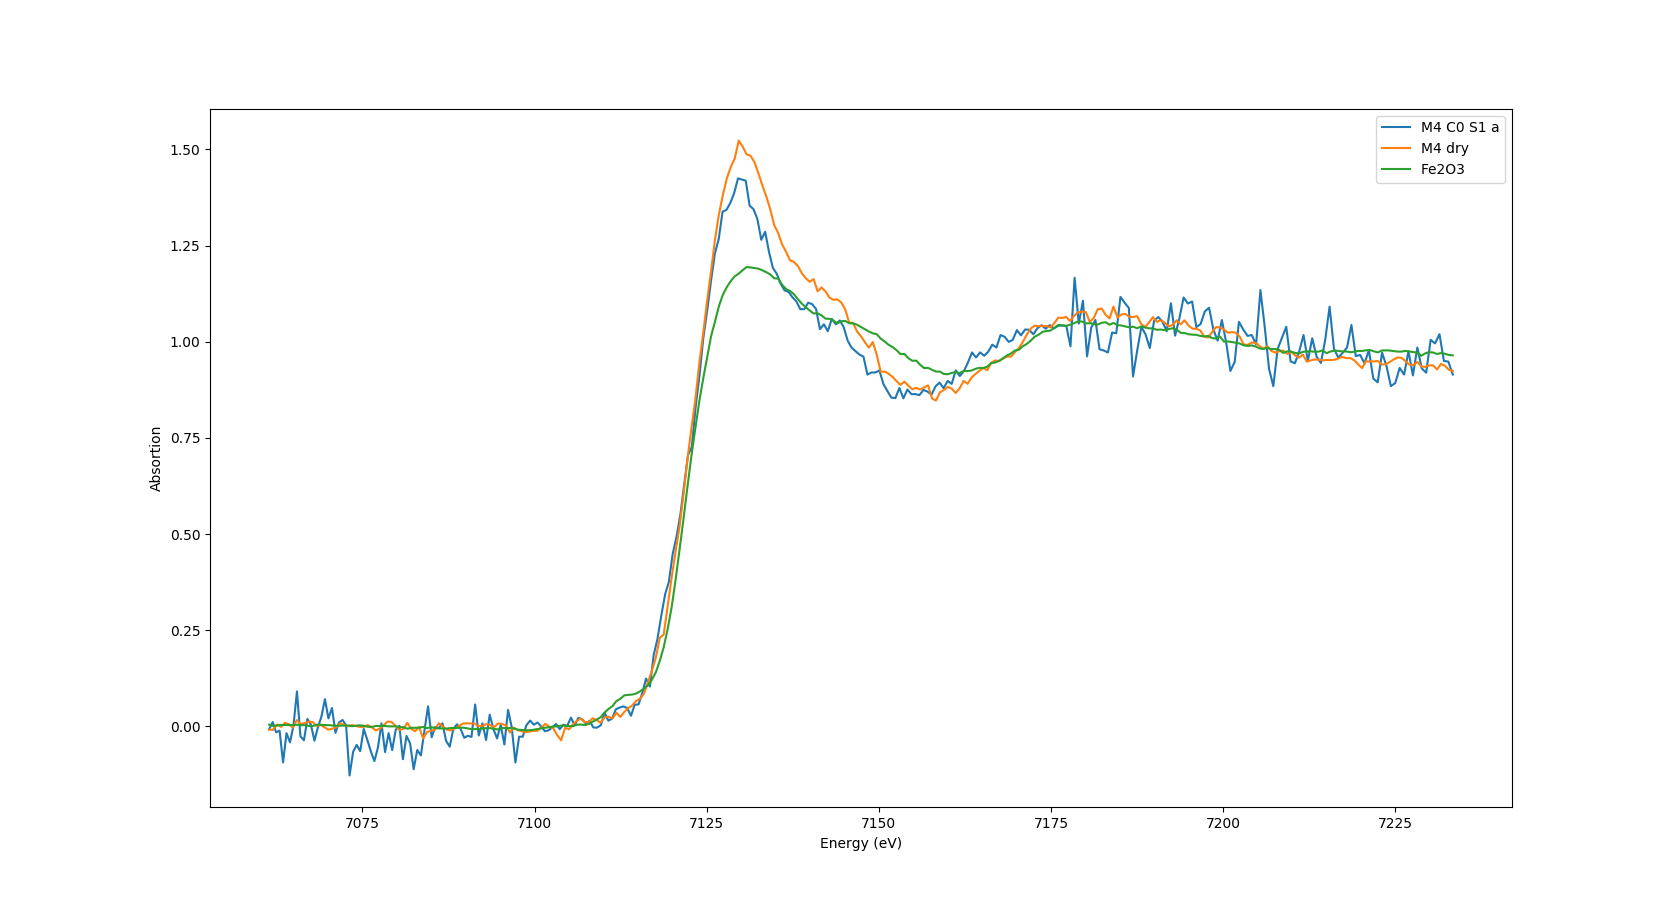
\includegraphics[width=0.9\textwidth]{../Kuvat/Sulfideja/M4_Fe2O3.png}
  \caption{M4 soil with no added \ch{C} after two months of incubation. The results are compared to the dry sample and \ch{Fe2O3} reference sample.}
\end{figure}

\begin{figure}[h!]
  \label{fig:M5_noC}
  \centering
    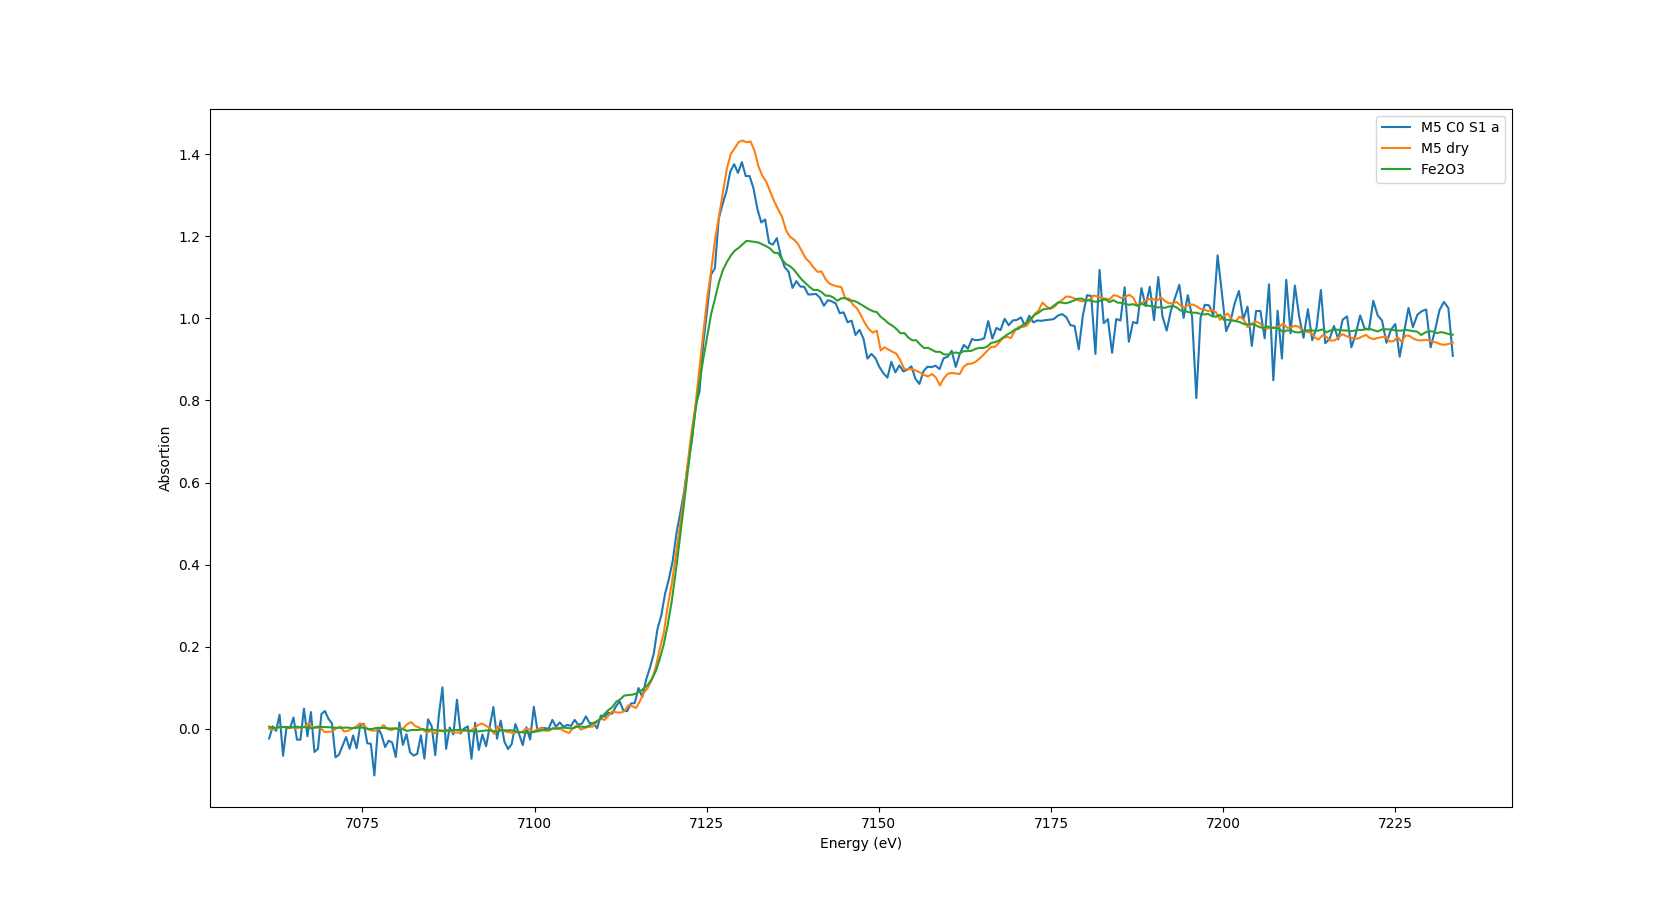
\includegraphics[width=0.9\textwidth]{../Kuvat/Sulfideja/M5_noC.png}
  \caption{M5 soil with no added \ch{C} after two months of incubation. The results are compared to the dry sample and \ch{Fe2O3} reference sample.}
\end{figure}

To gain better understanding of this result we performed a simulation of certain \ch{Fe} complexes. We used FDMNES software \cite{FDMNES} for these simulations, and the results are shown in figure \ref{fig:simu}.

\begin{figure}[h!]
  \label{fig:simu}
  \centering
     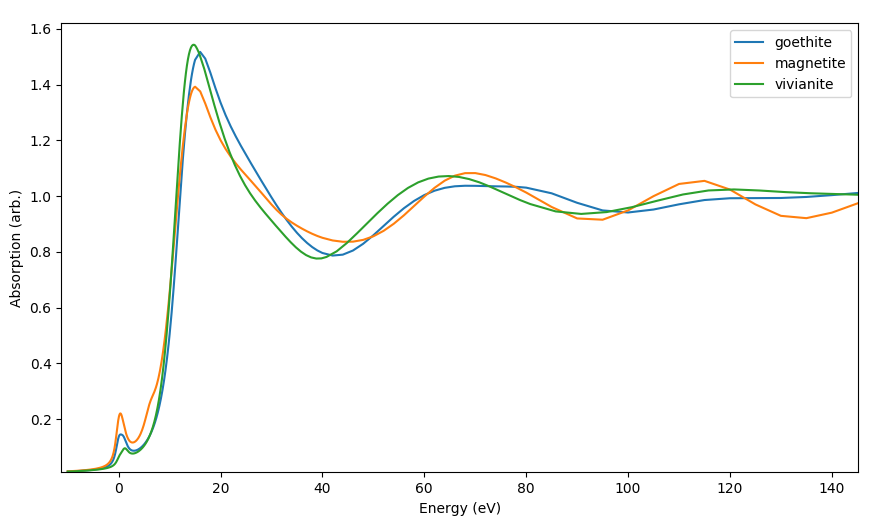
\includegraphics[width=\textwidth]{../Kuvat/mineral_spectra.png}
  \caption{Simulation results of our FDMNES simulation of a few \ch{Fe} minerals.}  
\end{figure} 
The simulation results indicate, that the new component present in our measurements is vivianite. Unfortunately we were not able to acquire unoxidised vivianite to be used as a reference for our measurements. In the literature we found one measurement, where both \ch{FeS} and vivianite were measured by Sulu-Gambari F. et al. \cite{Viv_spectra}. Their results are shown in figure \ref{}.

\begin{figure}[h!]
  \label{fig:Sulu}
  \centering
     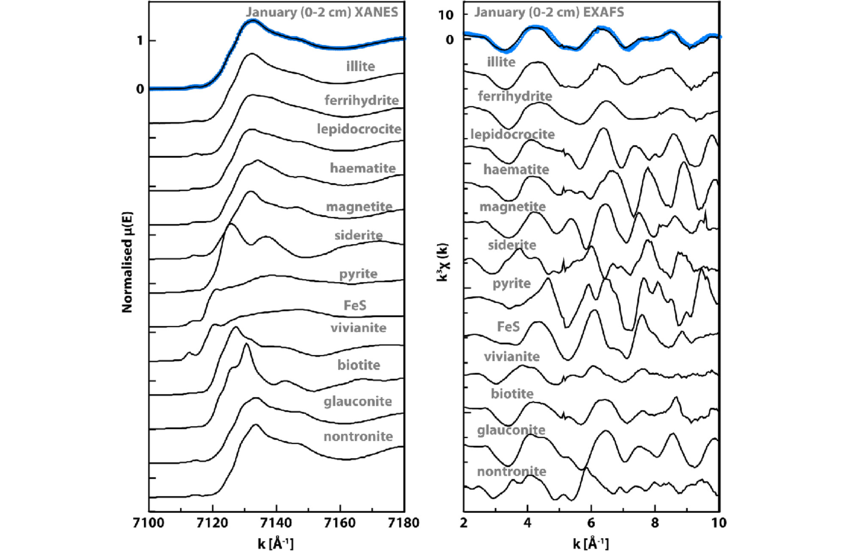
\includegraphics[width=\textwidth]{../Kuvat/vivianiitti_spectra.png}
  \caption{The measurement results of Fe K-XANES of certain Fe minerals from the literature \cite{Viv_spectra}.}
\end{figure}
These were measurements of their so called reference samples, and they did not specify was the sample oxidized or not. This makes the comparison with our samples difficult, since we want be to sure that the vivianite is unoxidized. This problem has to be tackled in future measurements, and we probably have make the unoxidized vivianite sample chemically in anaerobic environment, along with other iron oxyhydroxides.       
\subsubsection{Samples with added \ch{C}}
Similarly the samples with added \ch{C} were also stored in a cold and dark room for two months. The color of the soil was altered into black, which indicated that sulphides had been produced. The results shown figures \ref{fig:M1_C},\ref{fig:M2_C},\ref{fig:M4_C} and \ref{fig:M5_C}.
\begin{figure}[h!]
  \label{fig:M1_C}
  \centering
    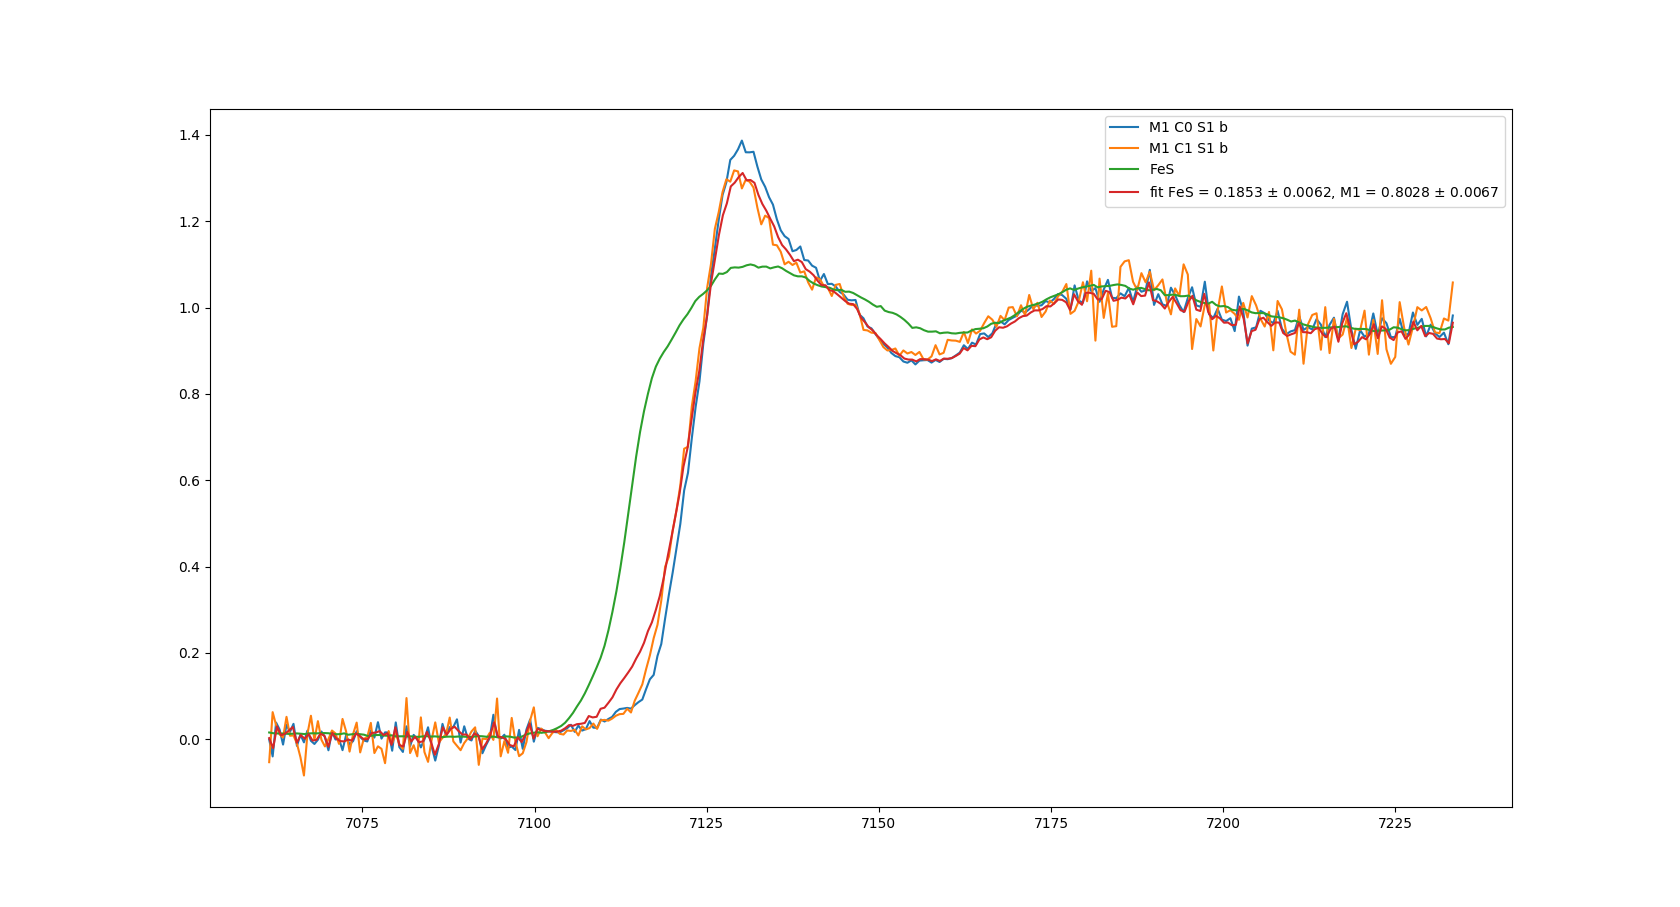
\includegraphics[width=0.9\textwidth]{../Kuvat/Sulfideja/M1_cauchy.png}
  \caption{M1 soil with added \ch{C} after two months of incubation, compared with \ch{FeS} reference and the case with no added \ch{C}}
\end{figure}

\begin{figure}[h!]
  \label{fig:M2_C}
  \centering
    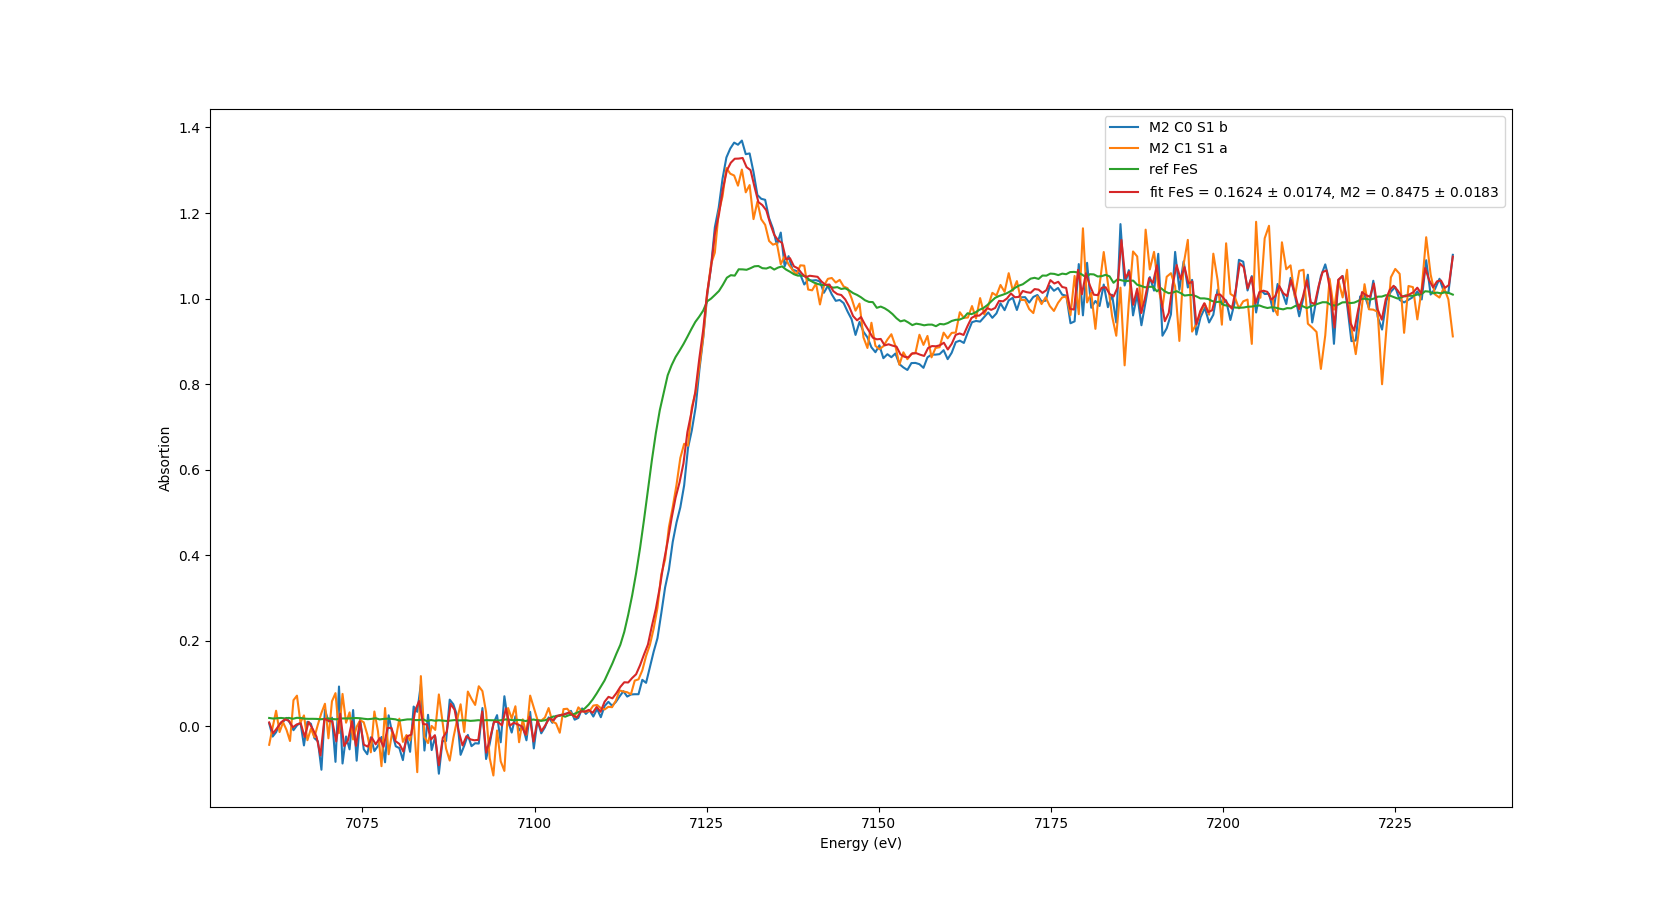
\includegraphics[width=0.9\textwidth]{../Kuvat/Sulfideja/M2_cauchy.png}
  \caption{M2 soil with added \ch{C} after two months of incubation, compared with \ch{FeS} reference and the case with no added \ch{C}.}
\end{figure}

\begin{figure}[h!]
  \label{fig:M4_C}
  \centering
    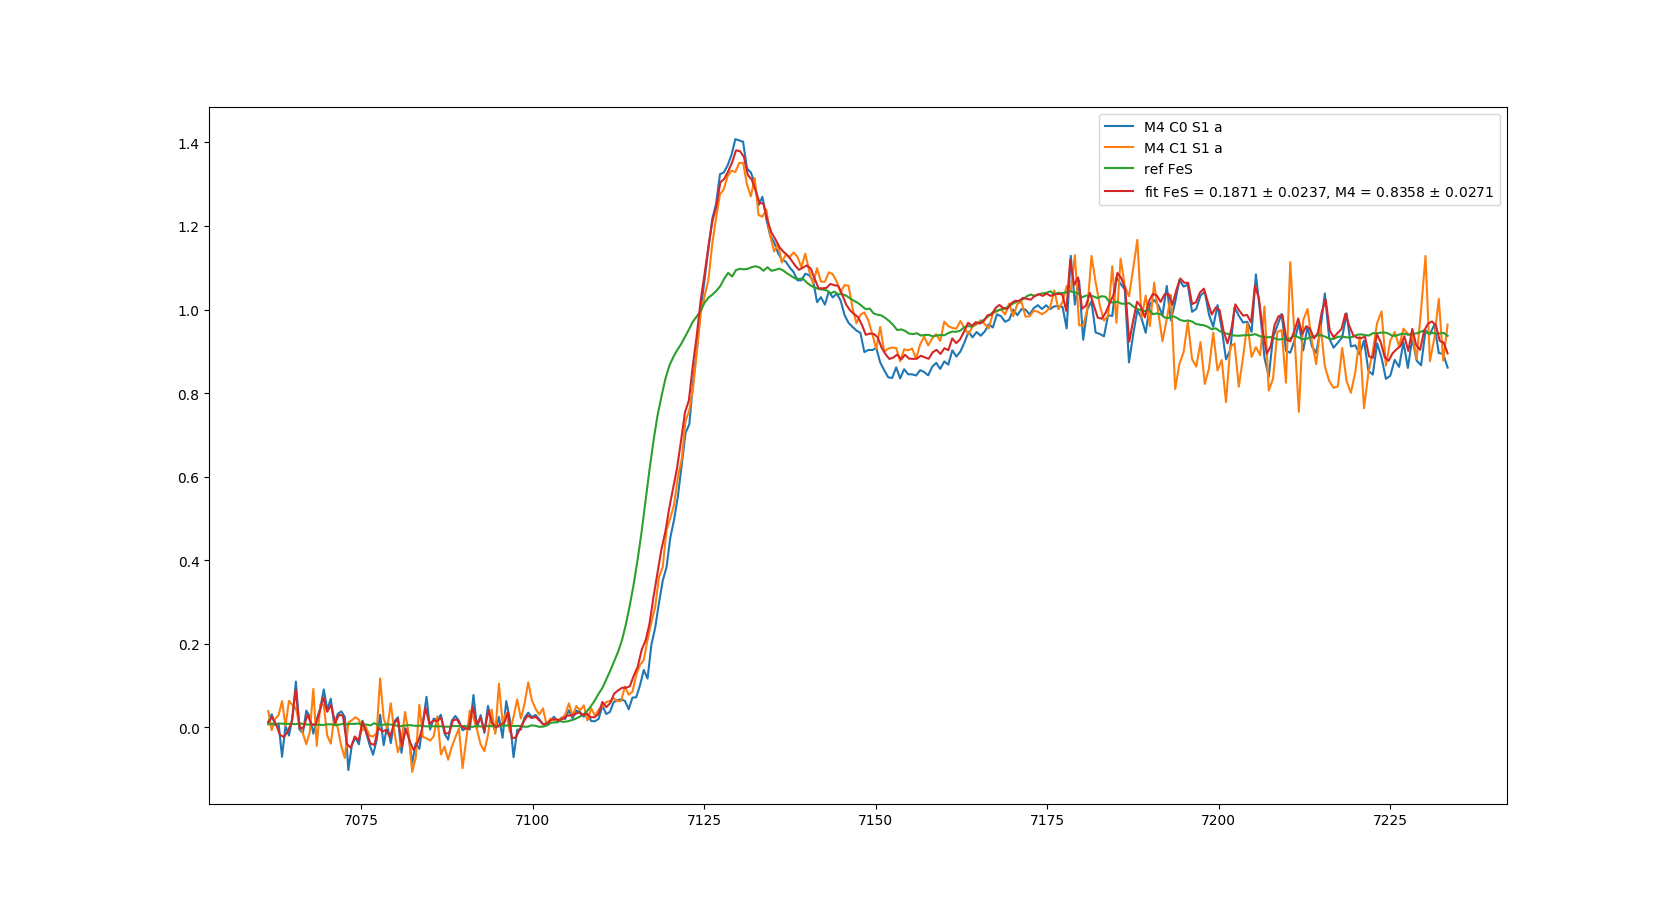
\includegraphics[width=0.9\textwidth]{../Kuvat/Sulfideja/M4_cauchy.png}
  \caption{M4 soil with added \ch{C} after two months of incubation, compared with \ch{FeS} reference and the case with no added \ch{C}.}
\end{figure}

\begin{figure}[h!]
  \label{fig:M5_C}
  \centering
    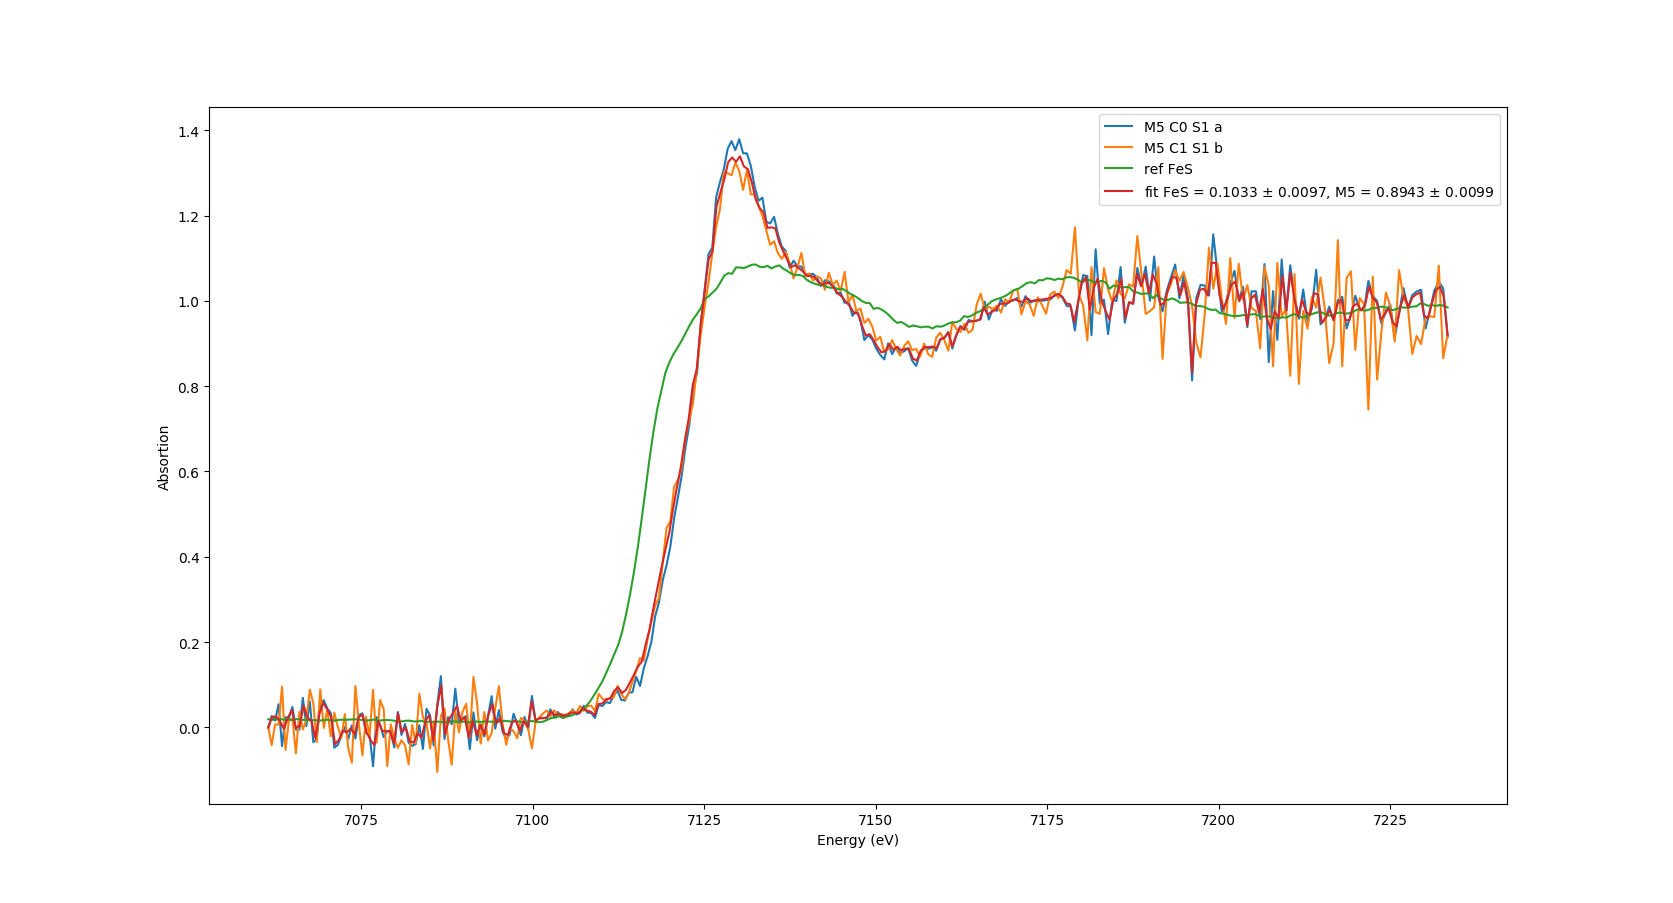
\includegraphics[width=0.9\textwidth]{../Kuvat/Sulfideja/M5_cauchy.png}
  \caption{M5 soil with added \ch{C} after two months of incubation, compared with \ch{FeS} reference and the case with no added \ch{C}.}
\end{figure}
We also measured the M3 soil, but our co-workers forgot to add the \ch{C}, so there was no change in the chemical state. However this further verifies, that adding organic \ch{C} indeed is needed for \ch{FeS} production to take place. The measurement result of M3 soil is displayed in figure \ref{fig:M3_C}.

\begin{figure}[h!]
  \label{fig:M3_C}
  \centering
    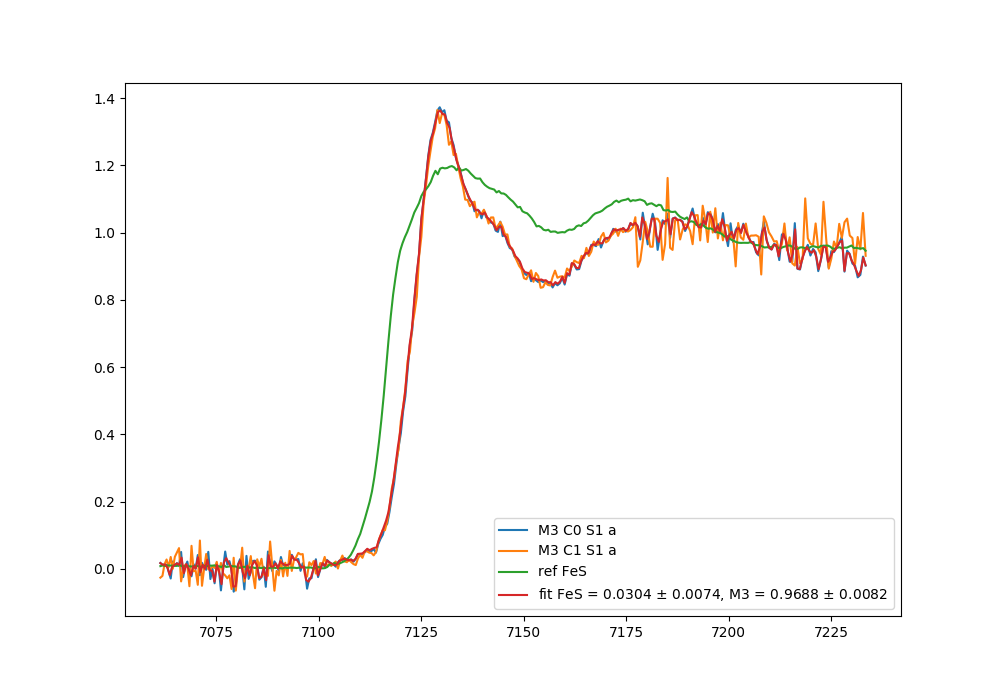
\includegraphics[width=\textwidth]{../Kuvat/Sulfideja/M3_alustava.png}
  \caption{M3 soil, where the \ch{C} was not added. There is little to non change in the chemical state.}
\end{figure}

The samples were compared compared with the samples with no added \ch{C} and a reference \ch{FeS} sample. Based on these we performed a least squares fit and also taking into account outlier point. As a result we noticed that sulphides had been formed as follows; M1: $\ch{FeS}=0.1853\pm0.01062$, M2: $\ch{FeS}=0.1624\pm0.0174$, M4:$\ch{FeS}=0.1871\pm0.0237$, M5:$\ch{FeS}=0.1033\pm0.0097$. 

\subsubsection{Samples with no \ch{S} and with no \ch{S} or \ch{C}}
The last set of measurements contained the anaerobic wet samples of M1 and M5 soils, where there was no \ch{S} in the sample. The other had the added \ch{C}. Results are shown in figures 

\begin{figure}[h!]
  \label{fig:M1_C0S0}
  \centering
    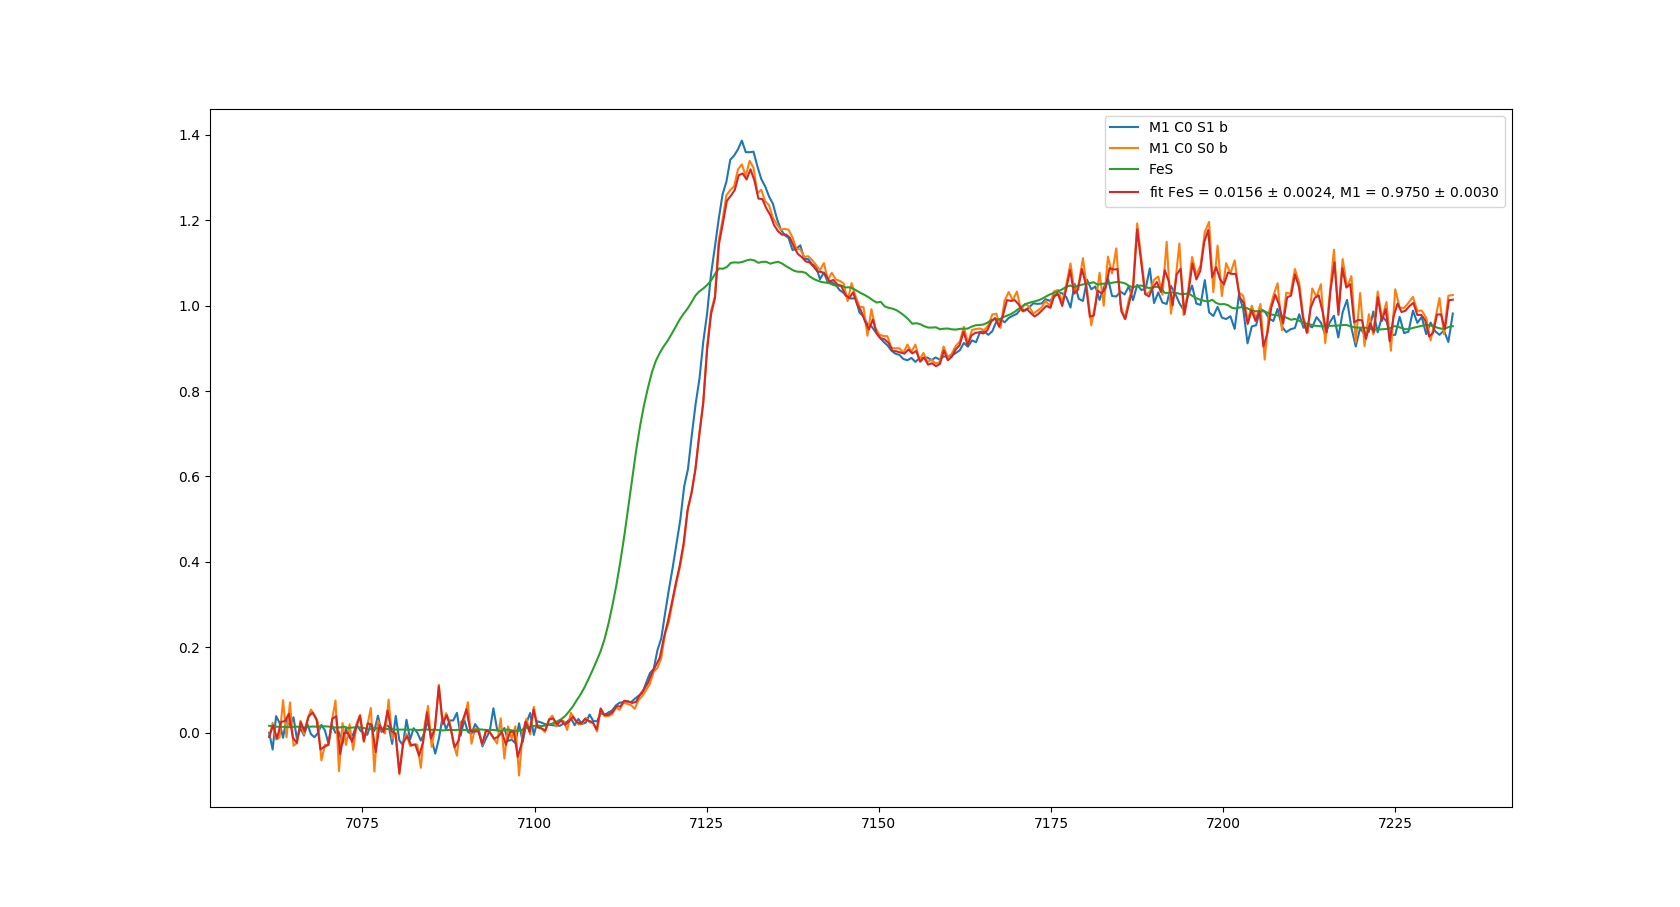
\includegraphics[width=0.9\textwidth]{../Kuvat/Sulfideja/M1C0S0b.png}
  \caption{M1 soil with no \ch{C} and no \ch{S} after two months of incubation, compared with \ch{FeS} reference and the case with no added \ch{C}.}
\end{figure}

\begin{figure}[h!]
  \label{fig:M5_C0S0}
  \centering
    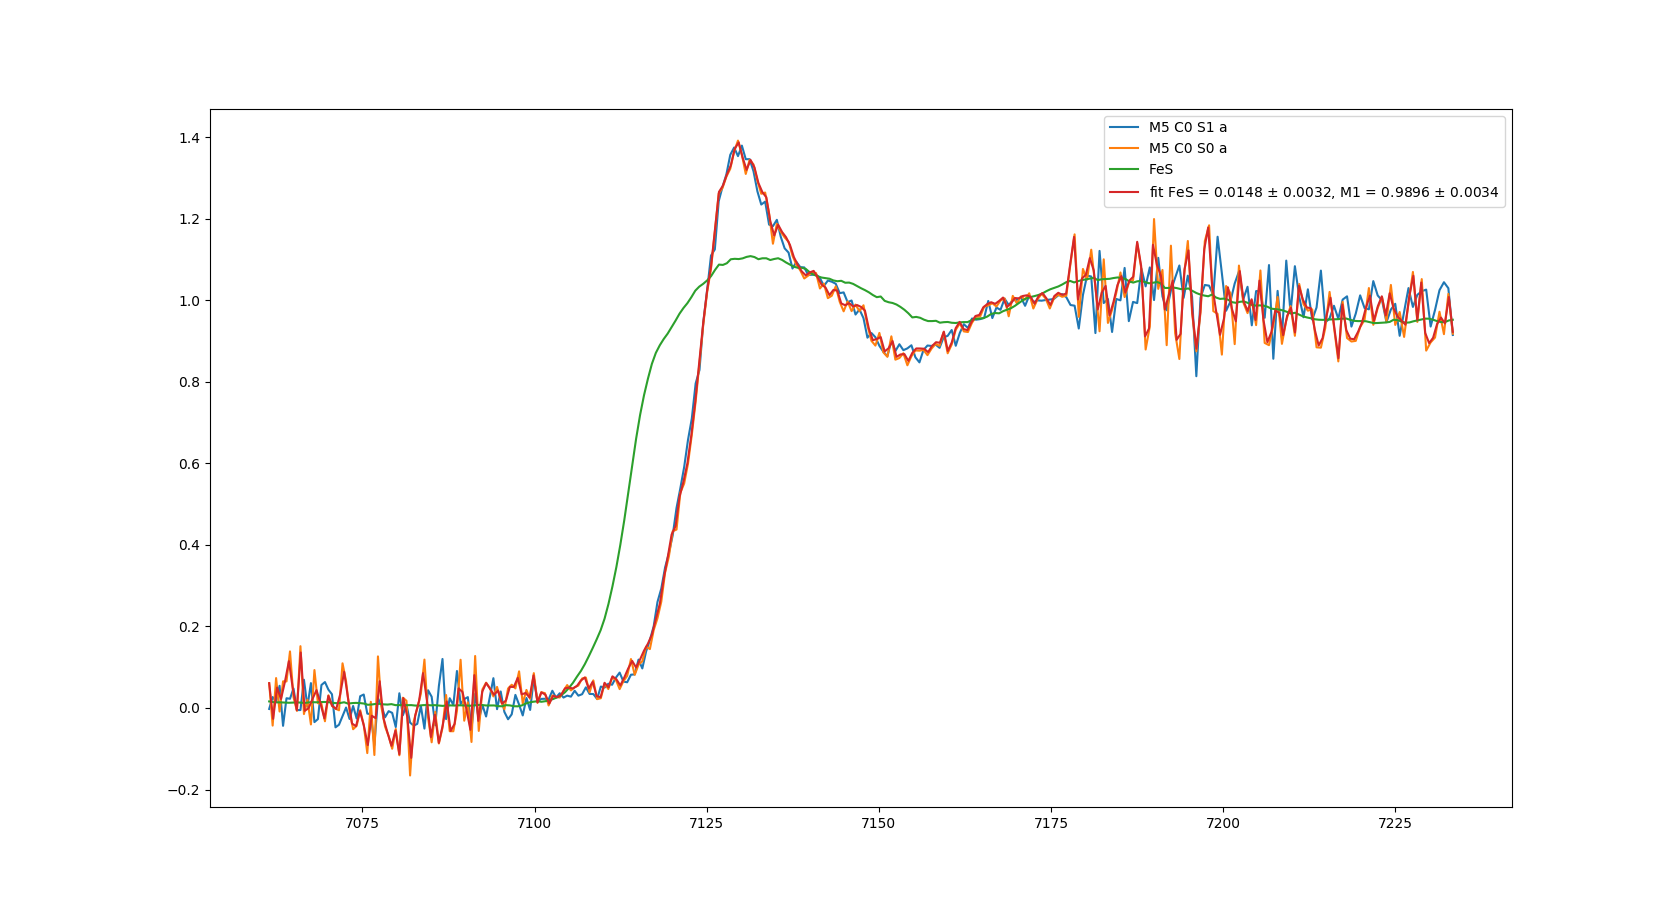
\includegraphics[width=0.9\textwidth]{../Kuvat/Sulfideja/M5C0S1a.png}
  \caption{M5 soil with no \ch{C} and no \ch{S} after two months of incubation, compared with \ch{FeS} reference and the case with no added \ch{C}.}
\end{figure}

\begin{figure}[h!]
  \label{fig:M1_C1S0}
  \centering
    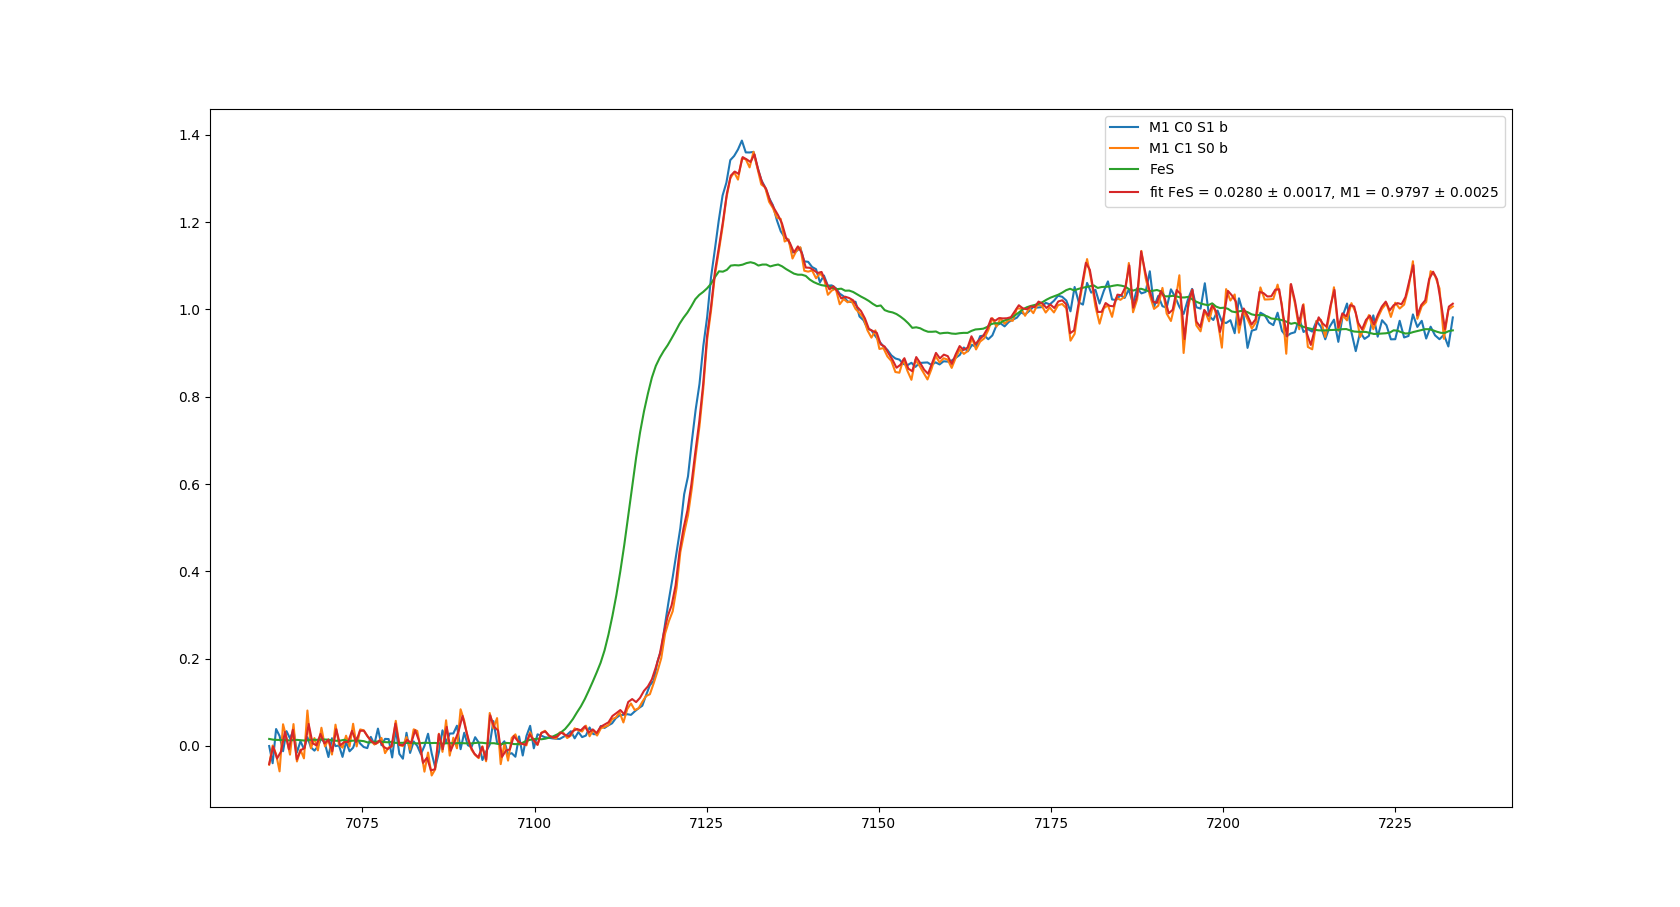
\includegraphics[width=0.9\textwidth]{../Kuvat/Sulfideja/M1C1S0b.png}
  \caption{M1 soil with the added \ch{C} and no \ch{S} after two months of incubation, compared with \ch{FeS} reference and the case with no added \ch{C}.}
\end{figure}

\begin{figure}[h!]
  \label{fig:M5_C1S0}
  \centering
    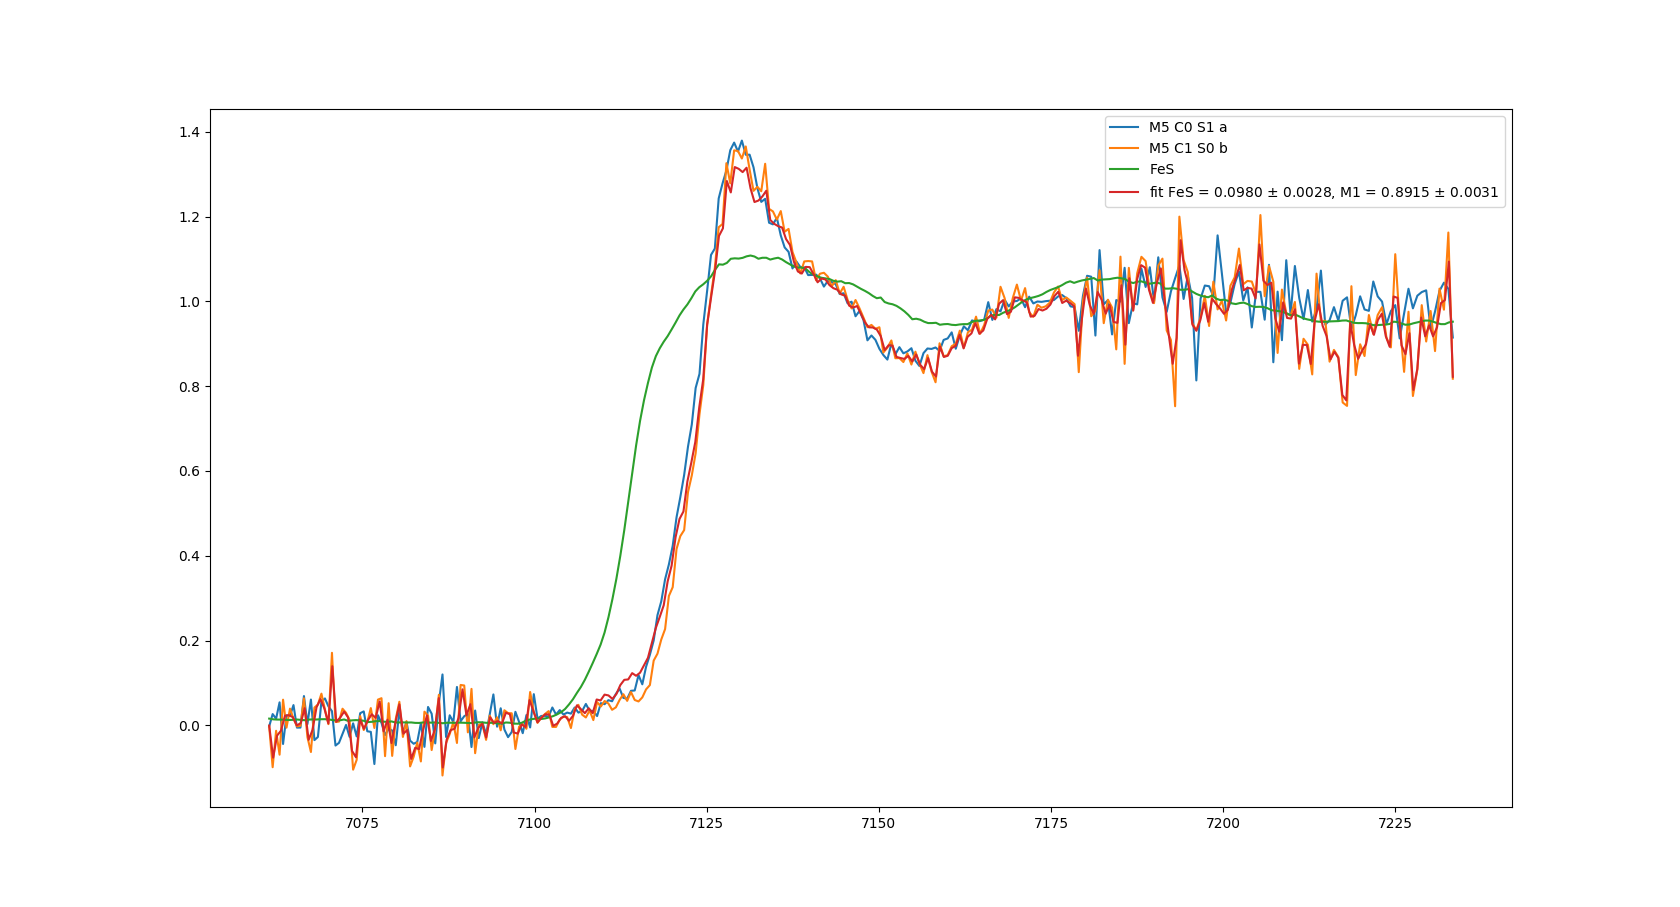
\includegraphics[width=0.9\textwidth]{../Kuvat/Sulfideja/M5C1S0b.png}
  \caption{M5 soil with the added \ch{C} and no \ch{S} after two months of incubation, compared with \ch{FeS} reference and the case with no added \ch{C}.}
\end{figure}
Now when there was no \ch{S} in the systems, we saw decreased sulphide levels compared to the samples with the added \ch{S}. For M1C0S0b sample we noted that the sample with added \ch{S} had $1.56\%\pm0.24\%$ more \ch{FeS}. M5C0S1a had $1.48\%\pm0.32\%$ more \ch{FeS} than M5C0S0a, M1C0S1b had $2.8\%\pm0.17\%$ more \ch{FeS} than M1C1S0b, and lastly M5C0S1a had $9.8\%\pm0.28\%$ more \ch{FeS} than M5C1S0b. It seem that some \ch{SO4} reduction takes place, if there is \ch{S} in the system, even without the added \ch{C}. 

\chapter{Conclusion}\label{conc}
In this work we developed a method to measure sediment samples in various conditions. We were able to measure and get meaningful results from our samples, and the method is easy to apply into other measurements as well.

%results
In our measurements we were able to verify that \ch{Fe} in our five different dry soils were mainly in \ch{Fe}(III) hydroxides. 24 hours after the soils were exposed to the water, the chemical state remained the same. After two months of incubation we started to see changes. The chemical state of the samples with no added \ch{C} was slightly altered, however we were not able to verify which \ch{Fe} mineral was formed, since none of our reference samples matched this result. Based on our simulations and literature, we expect this new mineral to be either vivianite, or some other unoxidised \ch{Fe} mineral. In case anaerobic samples with the added \ch{C}, we noticed the production of \ch{FeS}. In our samples the production of \ch{FeS} was between $10-20\%$, which indicates, that phosphorus stored in \ch{Fe}(III) oxides was released to the water. With no \ch{S} in the system, we saw smaller \ch{FeS} levels, between $1.5-10\%$ compared to the samples, with the added \ch{S} but no \ch{C}. This means that small amount of \ch{SO4} reduction takes place even without the added \ch{C}.  
%discussing the results

%future work
The method opens up possibilities for future work. With a larger amount of samples and with various water types one can form a more accurate picture of the sediment processes. The measurements could also be complimented with \ch{Mn} XANES studies and possibly even with \ch{P} studies on a synchrotron. With these additions to our result one could form a model of the sediment processes to be taken into account when planning the guidelines for erosion control measures around the Baltic sea and other water bodies vulnerable to eutrophication.

Another important measurement to complement our results would be to measure vivianite and other \ch{Fe} minerals, such as \ch{FeS2}. In order to measure the vivianite, it probably has to be self made chemically in an anaerobic environment to avoid oxidation. Also other minerals might be sensitive to oxidation, and it is possible that those are also present in our measurements.

All in all we were able to verify the production of sulphides under anoxic environment in our samples. This is in line with the model discussed in section 2.4. The sediment processes are currently taken into account in 

\begin{thebibliography}{9}

\bibitem{helcom}
Nutrient inputs to the Baltic sea, Baltic marine environment protection commission website,  
\url{http://www.helcom.fi/baltic-sea-trends/eutrophication/inputs-of-nutrients/}, cited 9.12.2018.

\bibitem{ymparisto}
Algal bloom monitoring 12.7.2018, Finland's environmental admistration  \url{http://www.ymparisto.fi/fi-FI/Vesi/Valtakunnallinen_levakatsaus_1272018_Sin(47369)}, cited 9.12.2018.

\bibitem{samassa}
Samassa vedess�, project website, \url{http://www.samassavedessa.fi/fi-FI}, cited 9.12.2018.

\bibitem{Fe concentration}
Chesworth W.
\textit{Geochemistry of micronutrients} In. Mortvedt, J.J., Cox, F.R., Shuman, L.M., Welch, R.M. (Eds.), \textit{Micronutriens in Agriculture}, Soil Science Society of America, Inc., Madison, Wisconsin, USA, pp. 1-30.

\bibitem{Soil erosion}
Petri Ekholm, Jouni Lehtoranta.
\textit{Does control of soil erosion inhibit aquatic eutrophication}.
Journal of Environmental Management 93 (2012) 140-146.

\bibitem{Labile carbon}
Lehtoranta J., Ekholm P., Wahlstr�m S., Tallberg P., Uusitalo R.
\textit{Labile organic carbon regulates phosphorus release from eroded soil transported into anaerobic coastal system}.
Ambio 2015, 44(Suppl. 2) 263-273.

\bibitem{Vivianite}
Reed D., Gustafsson B., Slomp C. \textit{Shelf-to-basin iron shuttling enhances vivianite formation in deep Baltic sea sediments}. Earth and Planetary Science Letters 434 (2016) 241-251. 

\bibitem{Ros}
Jilbert T., Asmala E., Schr�der C., Tiihonen R., Myllykangas J-P., Virtasalo J. J., Kotilainen A., Peltola P., Ekholm P., Hietanen S.
\textit{Impacts of flocculation on the distribution and diagenesis of iron in boreal estuarine sediments}.
Biogeosciences 15 (2018) 1243-1271. 

\bibitem{Elements}
Elements of Modern X-ray Physics, J. Als-Nielsen and D.McMorrow, John Wiley \& Sons, 2001.

\bibitem{Analyzer crystal}
Rovezzi M., Lapras C., Manceau A., Glatzel P., Verbeni R.
\textit{High energy-resolution x-ray spectroscopy at ultra-high dilution with spherically bent crystal analyzers of 0.5 m radius}.
Rev.Sci.Instrum.88 (2017) no.1

\bibitem{Optic alignment}
Mortensen D., Seilder G.
\textit{Robust optic alignment in a tilt-free implementation of Rowland circle spectrometer}.
Journal of Electron Spectroscopy and Related Phenomena, Volume 215, February 2017, Pages 8-15

\bibitem{Fundamentals}
Fundamentals of XAFS, Matthew Newville \url{https://web.archive.org/web/20110722032112/http://xafs.org/Tutorials?action=AttachFile&do=view&target=Newville_xas_fundamentals.pdf}

\bibitem{Viv_spectra}
Sulu-Gambari F., Seitaj D., Behrens T., Banerjee D., Meyesman F.J.R., Slomp C.P.,\textit{Impact of Cable Bacteria on Sedimentary Iron and Manganese Dynamics in a Seasonally-Hypoxic Marine Basin}, Geochemica et Cosmochimica Acta 192, July 2016.

\bibitem{FDMNES}
The FDMNES project website, 
\url{http://neel.cnrs.fr/spip.php?rubrique1007&lang=en}, cited 9.12.2018

\end{thebibliography}

\end{document}
